\documentclass[]{article}

%imports
\usepackage{amsmath}
\usepackage{amsthm}
\usepackage{amssymb}
\usepackage{tikz-cd}
\usepackage{tikz}
\usepackage{quiver}
\usepackage{array}
\usepackage[all,cmtip]{xy}



\usepackage{hyperref}
\usepackage{cleveref}


\usepackage[style=alphabetic]{biblatex}

%references
\addbibresource{ref.bib}
%\bibliography{ref.bib}

%newtheorems
\theoremstyle{definition}
\newtheorem{definition}{Definition}[section]

\newtheorem{theorem}{Theorem}[section]
\newtheorem{corollary}{Corollary}[section]
\newtheorem{lemma}{Lemma}[section]
\newtheorem{proposition}{Proposition}[section]
\newtheorem{example}{Example}[section]
\newtheorem{question}{Question}

%commands
\newcommand{\mo}{\ensuremath{\text{mod }}}
\newcommand{\rad}{\ensuremath{\underline{r}}}
\newcommand{\Hom}{\ensuremath{\text{Hom}}}
\newcommand{\tu}{\ensuremath{\tau}}
\newcommand{\Fac}{\ensuremath{\text{Fac }}}
\newcommand{\comment}[1]{}


\newcommand{\spmat}[1]{%
	\begin{bmatrix}#1\end{bmatrix}%
}




%opening
\title{Computing \tu-rigid modules}
\author{Håvard Utne Terland}

\begin{document}

%\maketitle

\section*{Sammendrag}
I denne masteroppgaven blir $\tau$-vippeteori, som først ble utviklet av av  Adachi, Iyama og Reiten i \cite{tau}, introdusert. Det blir så demonstrert hvordan teknikker fra \cite{Br_stle_2019}, samt kombinatoriske ideer kan anvendes i teorien.

Vi viser at mutasjonskoggeret av støtte-$\tu$-vippemoduler kan ha mer enn $2$ sammenhengende komponenter. Insipirert av en teknikk fra \cite{dij17} klassifiserer vi $\tau$-vippemoduler over en klasse algebraer med $2$ simple moduler, før vi til slutt diskuterer noen eksempler.
\newpage

\section*{Abstract}
In this thesis, we first give a brief introduction to $\tau$-tilting theory which was introduced by Adachi, Iyama and Reiten in \cite{tau}. We have particular focus on applying wall and chamber structures to understand the $\tau$-tilting theory of an algebra as in \cite{Br_stle_2019}.

Using the machinery from \cite{Br_stle_2019} and some combinatorial arguments, we give examples of algebras with more than $2$ components in their mutation quiver of support \tu-tilting pairs. We also classify the $\tau$-tilting modules for some specific classes of algebras with two simple modules using a technique inspired by \cite{dij17}.

\newpage
\section*{Acknowledgments}
I want to thank my main advisor, Prof. Aslak Bakke Buan, for guiding me through the field of representation theory, from Auslander-Reiten quivers to $\tau$-tilting. My co-advisor Prof. Øyvind Solberg has also been of great help. In particular, I am grateful for fruitful conversations on computational aspects of representation theory and for solid explanations on basic ring theory during my first semester at NTNU. I owe most of my intuition on module theory to meetings with Øyvind during the fall of 2019, and his detailed notes on non-commutative ring theory have been very useful.
I also want to thank Dr. Eric Hanson for very constructive feedback during the $\tau$-tilting theory seminars the spring of 2021.

I would also like to thank the algebra group at NTNU as a whole for welcoming me to the institute as a PhD candidate on the integrated PhD program and The Research Council of Norway for funding  ARTaC, the project on which I am employed.

Outside the university, I want to thank my friends in Skansegata that I lived with while writing this thesis; Andreas, Henrik, Halvor, Marius and Vegard. 

Lastly I want to thank my father Rune and his father Ole for inspiring me to study mathematics, and my mother Kristin and her father Edmund for supporting my pursuit of a career in academia.

\newpage


\tableofcontents
\newpage
\section{Introduction}
Representation theory of algebras may be thought of as understanding the ways a finite set of linear transformations could act together on vector spaces given some constraints. This can be formulated using the language of module theory, where systems of linear transformations corresponds to modules over a finite dimensional algebra depending on the network one studies. 
%To be more precise, the network is given as a quiver, and the constraints are given as an ideal of the path algebra over the quiver.


In these terms, representation theory of algebras seeks to classify modules over finite dimensional algebras. To give an example, we may consider the quiver $\Gamma$ below, where we work over the field $\mathbb{R}$. A representation of this quiver is simply a linear transformation between two finite dimensional real vector spaces. Such a representation corresponds to a finitely generated module over the algebra $k\Gamma \cong \begin{bmatrix}
	\mathbb{R} & 0 \\ \mathbb{R} & \mathbb{R}
\end{bmatrix}$.
% https://q.uiver.app/?q=WzAsMixbMCwwLCJcXGJ1bGxldCJdLFsxLDAsIlxcYnVsbGV0Il0sWzAsMV1d
\[\begin{tikzcd}
	\Gamma: 1 & 2
	\arrow[from=1-1, to=1-2]
\end{tikzcd}\]

A representation of $\Gamma$ is in other words given by an arbitrary $n \times m$ real matrix. When dealing with a single linear transformation, classical linear algebra is sufficient, and computing the rank, nullity and corank of the matrix gives us everything we need to understand the transformation (corank for an $n \times m$ matrix is $m$ minus the rank of the matrix). Thus, there is no surprise that there are three indecomposable representations of this quiver, as seen in \cref{example-a2-figure}. Any representation of $\Gamma$ given as a matrix $M$ can be written uniquely up to isomorphism as the sum $M_1^r \oplus M_2^n \oplus M_2^c$, where $r,n$ and $c$ correspond to rank, nullity and corank of $M$.

% https://q.uiver.app/?q=WzAsNixbMCwyLCJcXGJ1bGxldCJdLFsxLDIsIlxcYnVsbGV0Il0sWzAsMSwiXFxidWxsZXQiXSxbMSwxLCJcXGJ1bGxldCJdLFswLDAsIlxcYnVsbGV0Il0sWzEsMCwiXFxidWxsZXQiXSxbMCwxXSxbMiwzXSxbNCw1XV0=
\begin{figure}[h]
	\[\begin{tikzcd}
		M_1: k & k \\
		M_2: k & 0 \\
		M_3: 0 & k
		\arrow[from=3-1, to=3-2,"0"]
		\arrow[from=2-1, to=2-2,"0"]
		\arrow[from=1-1, to=1-2,"1"]
	\end{tikzcd}\]
\caption{The three indecomposable representations of the quiver with one arrow.}
\label{example-a2-figure}

\end{figure}

For more complicated algebras, finding all indecomposable modules can be challenging. However, Auslander-Reiten theory offers some useful tools. In particular, for algebras of finite representation type (i.e with only finitely many indecomposable modules up to isomorphism), one can compute all indecomposable modules algorithimcally. Indeed, all modules fit into a so-called AR (Auslander-Reiten) quiver. For algebras of finite representation type, it is well-known that this quiver must be connected. Since we know all projective modules, we can compute all projectives and simply traverse the AR-quiver of our algebra. These steps are of algorithmic nature and are implemented in \cite{qpa}.

More general algebras can have infinitely many indecomposable modules up to isomorphism and also uncountably many components in their AR-quiver. In fact, one can show that describing the modules over what are called "wild" algebras is as at least as difficult as classifying any other module category, in the sense that any module category can be embedded in the module category of a wild algebra. Other tools such as tilting theory therefore come into play, where the general idea is to use module categories of relatively well-understood algebras to say something about module categories over different algebras. 

The topic of this thesis is to understand support $\tu$-tilting modules, which unify some of the different "tilting-theories" that has been constructed. However, in this thesis we are not interested so much in the "tilting" aspect, but instead seek to classify support $\tu$-tilting modules as they themselves have become objects of independent interest.

Like indecomposable modules in an AR-quiver, maximal $\tu$-rigid modules fit into a combinatorial structure given by a quiver. Like AR-quivers, these objects may be computed. And for algebras with only finitely many $\tu$-rigid objects up to isomorphism, the underlying graph of the quiver must be connected. This gives one example of how algebras with finitely many $\tu$-rigid objects play a similar role in $\tu$-tilting theory as representation finite algebras play in classical representation theory.

In this thesis, our main results concern algebras with infinitely many $\tu$-rigid modules. For such algebras, many of the tools developed for $\tu$-tilting finite algebras fail and therefore new techniques are needed.



\section{Preliminaries}
We refer the reader to the two books \cite{assem_skowronski_simson_2006} and \cite{auslander_reiten_smalo_1995} for general representation theory of algebras. We here collect some prerequisites for this thesis not found in these two texts. 

\subsection{Notation and setting}
We closely follow the notation of \cite{assem_skowronski_simson_2006}. By an algebra $A$ we mean a finite dimensional algebra over a field $k$, where $k$ need not be algebraically closed. All algebras encountered in this thesis will be on the form $k\Gamma/I$ for some finite quiver $\Gamma$ and admissible ideal $I$. We denote by $r$ the ideal of $k\Gamma$ generated by all paths of length $1$ in $\Gamma$. By $\underline{r}$ we mean the image of $r$ under the canonical epimorphism $k\Gamma \to k\Gamma/I$. The number $n$ is, unless otherwise stated, reserved for the number of indecomposable projective summands of $A$. By $\mo A$ we denote the category of finite dimensional left $A$-modules (in contrast to \cite{assem_skowronski_simson_2006}, who employ right modules). We implicitly identify $kQ/I$-modules with its representation over the bound quiver $Q$ with relations $I$. For the algebra $k\Gamma/I$, there is for all vertices $i$ in $\Gamma$ an associated indecomposable projective module $P(i)$ generated by all finite paths starting in that vertex. Similarly, $I(i)$ is the associated injective module for vertex $i$.

Fix an algebra $A = k\Gamma/I$ with $n$ simple modules. For a module $M$ over $A$, we denote by $[M]$ the dimension vector of $M$. For such a dimension vector to be well-defined, an implicit order of the vertices of $\Gamma$ is needed. The dimension vector of $S(i)$ is then for example $(0,\dots,0,1,0,\dots,0)$ with $1$ in the $i$th position. A useful theoretical framework for dealing with  dimension vectors is the Grothendieck group $K_0(A) \cong \mathbb{Z}^n$ with basis $([S(1)],[S(2)],\dots,[S(n)])$. We refer the reader to\cite{assem_skowronski_simson_2006} for a rigorous definition. 


We denote by $D$ the duality on modules. For an $A$-module $M$, we denote by $M^*$ the  $A^\text{op}$-module given by $\text{Hom}_A(M,A)$. For the indecomposable projective module over $A$ in vertex $i$ we have that $P(i)^*$ will be the indecomposable projective module over $A^\text{op}$ also in vertex $i$. We denote by $\text{Tr}$ the transpose. The Auslander-Reiten translate $D\text{Tr}$ is denoted $\tau$.

A module $M$ over $A$ is called basic if no two nonzero summands are isomorphic as $A$-modules, that is $M \cong Y \oplus X \oplus X$ implies $X \cong 0$. We denote by $|M|$ the number of indecomposable summands of $M$. 

We denote by $hom_A(M,N)$ the dimension of the $k$-vector space $\text{Hom}_A(M,N)$.

Given a subcategory $\mathcal{C}$ of $\text{mod } A$, the right-perpendicular category of $\mathcal{C}$, denoted $\mathcal{C}^\perp$ is defined as the subcategory of all modules $M$ such that $\text{Hom}_A(C,M) = 0$ for all $C \in \mathcal{C}$. Dually, the left perpendicular of $\mathcal{C}$, denoted $^{\perp}\mathcal{C}$ is defined as the subcategory of all modules $M$ such that $\text{Hom}_A(M,C) = 0$ for all $C \in \mathcal{C}$. Given a module $M$, we define $\text{add } M$ to be the subcategory of $\text{mod } A$ consisting of all modules $N$ such that all indecomposable summands of $N$ are summands of $M$. 

\subsection{Approximations}
Approximations are very often used in \tu-tilting theory, for example to compute mutations which are central to this thesis.

\begin{definition}
	Let $\mathcal{C}$ be a subcategory of $\text{mod}  A$.  Let $M$ be an $A$-module, and $X \in \mathcal{C}$. A map $f:X \to M$ is called a \textit{right $\mathcal{C}$-approximation} of $M$ if it is the case that for any $Y \in \mathcal{C}$ and map $g:Y \to M$, there is a map $h:Y \to X$ such that $g = f \circ h$. 
	
	Let $M$ be an $A$-module, and $X \in \mathcal{C}$. A map $f:M \to X$ is called a \textit{left $\mathcal{C}$-approximation} of $M$ if it is the case that for any $Y \in \mathcal{C}$ and map $g:M \to Y$, there is a map $h:X \to Y$ such that $g = h \circ f$. 
	
	A left (right) approximation which is also left (right) minimal as a map is called a minimal left (right) approximation.
	
	If $\mathcal{C} = \text{add } M$ for a module $M$, we shorten $\text{add }M$-approximation to $M$-approximation.
\end{definition}


We say that a subcategory $\mathcal{C}$ of $\text{mod }A$ is \textit{contravariantly finite} (resp. \textit{covariantly finite}) if every $A$-module $M$ has a right (resp. left) $\mathcal{C}$-approximation. If $\mathcal{C}$ is both contravariantly and covariantly finite, we call it \textit{functorially finite}.


\begin{example}
	Let $M,N$ be modules in $\text{mod } A$. We may always find a left $M$-approximation of $N$ as follows. $\text{Hom}(N,M)$ is finite dimensional as a $k$-vector space, so pick a basis $F = (f_1,f_2,\dots,f_i)$. Then we have a map $f:N \to \bigoplus_{j= 1}^i M$ given by $f = \begin{bmatrix}
	f_1 \\ \vdots \\ f_i
	\end{bmatrix}$. Given any map $g_r:N \to \bigoplus_{j = 1}^k M_j$ where $M_j$ is a summand of $M$, this map will naturally factor through a map $g:N \to \bigoplus_{j = 1}^k M$, which we may describe as $g = [g_1,g_2,\dots,g_k]$. Since $F$ is a basis for $\text{Hom}(M,N)$, we may write \[g = [a_{1,1}f_1 + \dots + a_{1,i}f_i,\dots,a_{k,1}f_1 + \dots + a_{k,i}f_i]\]
	
	Interpreting $c \in k$ as a map $M \to M$ given by $c \cdot1$ where $1$ is the identity map, we can write $g$ as the composition
	\[g = \begin{bmatrix}
	a_{1,1} & \dots & a_{1,i} \\
	\vdots & \dots & \vdots \\
	a_{k,1} & \dots & a_{k,i}
	\end{bmatrix} \times \begin{bmatrix}
	f_1 \\ \vdots \\ f_i
	\end{bmatrix}
	\]
	
	and thus $g_r$ also factors through as wanted.
\end{example}

We now give an example of a non-trivial, non-minimal left approximation.

\begin{example}
	Let $A$ be the algebra defined by the quiver
	\[
	\begin{tikzcd}
	1 \arrow[r,bend left,"\alpha"] & 2 \arrow[l,bend left,"\beta"]  \\
	\end{tikzcd}
	\]
	modulo the relations $r^4 = 0$. Then $\text{Hom}(P(1),P(2))$ has dimension $2$, with maps $f_1(x) = x \beta$ and $f_2(x) =  x\beta\alpha\beta$. Clearly, $f_2 = (\beta\alpha) \circ f_1$. 
	
	Using the construction in the above example, the map $f = \begin{bmatrix} \beta \\ \beta\alpha\beta \end{bmatrix}$ is a left $P(2)$-approximation of $P(1)$. It is not left minimal, however. To see this, consider the endomorphism on $P(2) \oplus P(2)$ given by \[\phi = \begin{bmatrix} 1 & 0 \\ \alpha\beta & 0\end{bmatrix}\]
	
	Then $\phi \circ f = f$, but $\phi$ is not an isomorphism. In fact, $f_1$ is a minimal left approximation.
\end{example}


\section{Tau-tilting theory}
$\tau$-tilting theory was introduced in \cite{tau} as a possible generalization of tilting theory, which itself has had tremendous impact on the field of representation theory of finite dimensional algebras. Although first introduced in \cite{tau}, some of the main results of $\tau$-tilting theory stem from work by Auslander and Smalø in the 80's, for example \cite{auslandersmalo81}. In this section, we recall some important definitions and results from $\tau$-tilting theory. 

We start by discussing $\tau$-rigid modules, which may be considered the building blocks of $\tau$-tilting theory. 


\begin{definition}
	A module $M$ in $\mo A$ is called $\tau$-rigid if $\Hom(M,\tau M) = 0$.
\end{definition}

First note that the Auslander-Reiten formula gives that \tu-rigid objects must have no self-extensions, that is, they are exceptional objects. Note also that $X,Y$ being $\tau$-rigid does not imply $X \oplus Y$ being $\tau$-rigid. In fact, studying how indecomposable $\tau$-rigid modules together form larger $\tau$-rigid modules is part of $\tau$-tilting theory.

\begin{definition}\cite[Definition 0.3]{tau}
	A pair $(M,P)$ where $M$ is basic $\tau$-rigid and $P$ basic projective such that $\Hom_A(P,M) = 0$ is called a  $\tau$-rigid pair.
\end{definition}

Along with this definition follows many conventions. Fix a  $\tau$-rigid pair $T = (M,P)$. By the projective part of $T$ we mean $P$, and by the module part of $T$ we mean $M$. $T$ is called support \tu-tilting if $|M| + |P| = n$, and almost complete support \tu-tilting if $|M| + |P| = n - 1$.

\begin{proposition}\cite[Proposition 1.2, Proposition 2.3]{tau}
	A basic $\tu$-rigid pair over $A$ has at most $n = |A|$ summands.
\end{proposition}

The above proposition shows that support $\tu$-tilting pairs really are "complete". A support \tu-tilting pair with zero projective part may also be denoted a \tu-tilting module. 




For $T_1,T_2$ both \tu-rigid pairs, we consider $T_1$ a summand of $T_2$ is both the module part and the projective part of $T_1$ is a summand of the module part and the projective part of $T_2$ respectively.




\begin{example}
	Since $\tu P = 0$ for any projective module $P$, any projective module is \tu-rigid. As a consequence, $A = \oplus_{i = 1}^n P(i)$ is a \tu-tilting module.	
\end{example}

\begin{example}
	For an hereditary algebra $A$, partial tilting modules coincide with \tu-rigid modules. For $M$ partial tilting, $0 = Ext^1_A(M,M) \cong D\Hom_A(M,\tu M)$, where the first equality is part of the definition of tilting-modules and the second equality follows from the Auslander-Reiten formula in the hereditary case.
\end{example}

\subsection{Torsion pairs induced by support \tu-tilting pairs}

Given a support \tu-tilting pair $(M,P)$, we consider the subcategory  $\Fac M$ of modules generated by $M$. As in classical tilting theory, this is a torsion class.

\begin{definition}
	A pair $(\mathcal{T},\mathcal{F})$ of full subcategories of $\text{mod } A$ for an algebra $A$ is called a torsion pair if $\mathcal{T} = ^\perp\mathcal{F}$ and $\mathcal{F} = \mathcal{T}^\perp$. 
	
	A torsion class is the left part of a torsion pair, as $\mathcal{T}$ above. A torsion-free class is the right part of a torsion pair, as $\mathcal{F}$ above.
\end{definition}

Torsion pairs appear in classical tilting theory. Using the more general setting of $\tu$-tilting theory we can classify all functorially finite torsion pairs, i.e torsion pairs where both the torsion and torsion-free parts are functorially finite.

\begin{theorem}\cite[Theorem 2.7]{tau}
	There is a bijection between the set of functorially finite torsion pairs, denoted $\text{f-tors} A$ and support \tu-tilting pairs, denoted $\text{s}\tu\text{-tilt} A$, given by sending a support \tu-tilting pair $(M,P)$ to $(\Fac M,M^\perp)$.
\end{theorem}

We order the objects in $\text{f-tors} A$ by inclusion on the torsion classes. Thus $(X_1,Y_1) < (X_2,Y_2)$ if $X_1 \subseteq X_2$. This induces an ordering on the set of support \tu-tilting pairs, where $(M_1,P_1) < (M_2,P_2)$ if $\text{Fac}(M_1) \subset \text{Fac}(M_2)$.

 We denote by $Q(\text{f-tors} A)$ the Hasse-quiver of the above defined ordering on $\text{f-tors} A$.

\subsection{Mutation of support \tu-tilting pairs}
An essential property of support \tu-tilting pairs is that one can \textit{mutate} at each summand. More precisely, we have the following.

\begin{theorem}
	For a almost complete support $\tau$-tilting pair $(M,P)$, there exists exactly two distinct support \tu-tilting pairs $(M_0,P_0)$ and $(M_1,P_1)$ containing $(M,P)$ as a summand.
\end{theorem}

In the above theorem, $(M_0,P_0)$ and $(M_1,P_1)$ are said to be mutations of each other, and we may write $M_1 = \mu_X(M_0)$ where $X$ is the indecomposable summand of $M_0$ that we must replace to get $M_1$; formally, we require $M_0 = X \oplus M$ or $P_0 = X \oplus P$. In this case, we \textit{mutate} at $X$.

\begin{proposition}\cite[Definition-Proposition 2.28]{tau}
	Let $T_1$ and $T_2$ be support \tu-tilting pairs which are mutations of each other. Then either $T_1 < T_2$ or $T_ 2 < T_1$. In the first case, we consider $T_2$ a right-mutation of $T_1$ and in the second case we consider $T_2$ a left-mutation of $T_1$. Note that if $T_2$ is a left-mutation of $T_1$ if and only if $T_1$ is a right-mutation of $T_2$.
\end{proposition}

Left-mutations may be computed using approximations.

\begin{proposition}\cite[Theorem 2.30]{tau},\cite[Theorem 1.2]{zhang2016mutation}
	Let $T = X \oplus U$ be $\tau$-tilting and $X$ indecomposable such that $T$ is the Bongartz completion of $U$. Let \[X \xrightarrow[]{f} U' \to Y \to 0\] be exact, where $f$ is a minimal left 
	$\text{add } U$-approximation. 
	\begin{enumerate}
		\item  If $Y = 0$, then $U$ is the module part of some support \tu-tilting pair.
		\item If $Y \neq 0$, then $Y$ is indecomposable, and $U \oplus Y$ is $\tu$-tilting.
	\end{enumerate}

\end{proposition}

The following observation is practical for computational reasons as it demonstrates that we need not compute Bongartz completions before mutating; it is sufficient to check that the resulting $Y$ defines a new \tu-tilting object. 

\begin{proposition}
Let $T = X \oplus U$ be $\tau$-tilting. Let \[X \xrightarrow[]{f} U' \to Y \to 0\] be exact, where $f$ is a minimal left $\text{add } U$-approximation. 

If $Y \neq 0$, and $U \oplus Y$ is $\tu$-rigid, $Y$ must decompose as $Y = \bigoplus_{i = 1}^k Y'^i$. Then $U \oplus Y'$ is $\tu$-tilting.

\end{proposition}

\begin{proof}
	If $U \oplus Y$ is \tu-rigid with at least $n$ summands, then since $U$ is basic with $n-1$ summands, $Y$ must decompose as $Y = \oplus_{i = 1}^k Y'$ for some $k \geq 1$. $U \oplus Y'$ must then $\tu$-tilting and a mutation of $U \oplus X$, since they differ on exactly one summand.
\end{proof}

\subsection{Mutation quivers}
Mutation of support \tu-tilting modules naturally induce a quiver structure on the set of these modules.

\begin{definition}\cite[Definition 2.29]{tau}
	Fix an algebra $A$. The support $\tau$-tilting quiver $Q(\text{s\tu-tilt} A)$ has a vertex for each support \tu-tilting pair and arrows on the form $T_1 \to T_2$, where $T_2$ is a left mutation of $T_1$. 
\end{definition}

In the remaining of this subsection, we give examples of mutation quivers and discuss some elementary facts about them.


\comment{
Mutation of support \tu-tilting pairs is compatible with the ordering induced by the set of functorially finite torsion classes.
\begin{proposition}
	$Q(\text{s\tu-tilt} A)$ is isomorphic to $Q(\text{f-tors} A)$.
\end{proposition}

\begin{proof}
	We have an isomorphism between the vertex sets of the two quivers. It is enough to prove that there is an arrow $(T_1,P_1) \to (T_2,P_2)$ if and only if there is an arrow $(\Fac T_1,T_1^\perp) \to (\Fac T_2,T_2^\perp)$.
	
	If there is an arrow $(\Fac T_1,T_1^\perp) \to (\Fac T_2,T_2^\perp)$, we have $\Fac T_2 \subset \Fac T_1$ and no functorially finite torsion class $T \neq T_1,T_2$ such that $\Fac T_2 \subset T \subset \Fac T_1$. By \cite[Theorem 2.33]{tau}, this implies that $(T_2,P_2)$ is a left mutation of $(T_1,P_1)$ and thus there is an arrow $(T_1,P_1) \to (T_2,P_2)$ in $Q(\text{s\tu-tilt} A)$.
	
	By \cite[Theorem 2.33]{tau}, a symmetrical argument proves the other direction.	
\end{proof}


\begin{example}
	For any algebra $A$, $\Fac A=\text{mod } A$, the support \tu-tilting module $(A,0)$ is the largest element in $Q(\text{f-tors} A)$, and any mutation $\mu_X(A)$ must be a left-mutation.
\end{example}
}

\begin{example}
	Let $A$ be the path algebra of the disconnected quiver with two points.
	
	\[
	\begin{tikzcd}
	\bullet & \bullet   \\
	\end{tikzcd}
	\]
Then $Q(s\tau\text{-tilt} A)$ may easily be computed to be 

% https://q.uiver.app/?q=WzAsNCxbMSwwLCIoUCgxKVxcb3BsdXMgUCgyKSwwKSJdLFsxLDIsIigwLFAoMSlcXG9wbHVzIFAoMikpIl0sWzIsMSwiKFAoMSksUCgyKSkiXSxbMCwxLCIoUCgyKSxQKDEpKSJdLFswLDNdLFszLDFdLFswLDJdLFsyLDFdXQ==
\[\begin{tikzcd}
& {(P(1)\oplus P(2),0)} \\
{(P(2),P(1))} && {(P(1),P(2))} \\
& {(0,P(1)\oplus P(2))}
\arrow[from=1-2, to=2-1]
\arrow[from=2-1, to=3-2]
\arrow[from=1-2, to=2-3]
\arrow[from=2-3, to=3-2]
\end{tikzcd}\]
\end{example}

A crucial example which is needed for many of the main results in this thesis is the \tu-tilting theory of the Kronecker algebra $K$. The mutation quiver of $K$ is given in for example \cite{jassoreduction} and is considered to be well-known. For completeness, we include here a brief explanation of its $\tu$-tilting theory. For rigorous proofs that the modules we exhibit in fact are $\tu$-rigid (exceptional is sufficient in the hereditary case) we refer the reader to \cite[Chapter 9.2]{assem_skowronski_simson_2006}.
\begin{example}
Consider the Kronecker algebra $K$, which has quiver as drawn below.
% https://q.uiver.app/?q=WzAsMixbMCwwLCIxIl0sWzEsMCwiMiJdLFswLDEsIiIsMCx7Im9mZnNldCI6LTF9XSxbMCwxLCIiLDIseyJvZmZzZXQiOjF9XV0=
\[\begin{tikzcd}
	1 & 2
	\arrow[shift left=1, from=1-1, to=1-2]
	\arrow[shift right=1, from=1-1, to=1-2]
\end{tikzcd}\]

We will compute the mutation quiver $Q(s\tau\text{-tilt } K)$. $(K,0)$ and $(0,K)$ are support \tu-tilting modules. Since $K$ is hereditary, this is equivalent to finding all (support) tilting modules over $K$.

Since $\text{Hom}_K(P(1),P(2)) = 0$, $(P(2),P(1))$ is a support \tu-tilting pair which is a left mutation of $(K,0)$ and a right mutation of $(0,K)$.

The postprojective modules are $\tu$-rigid, and in fact \begin{align*}
	T^1_i = \tau^{-i}P(1) \oplus \tau^{-(i+1)}P(2) && T^2_i = \tau^{-i}P(1) \oplus \tau^{-i}P(2)
\end{align*}
define two classes of $\tau$-tilting modules, where we let $i \in \mathbb{N}$. See \cref{preprojective-K} for an illustration of the postprojective component.


\begin{figure}[h]
	% https://q.uiver.app/?q=WzAsNyxbMCwxLCJQKDIpIl0sWzEsMCwiUCgxKSJdLFsyLDEsIlxcdGF1XnstMX1QKDIpIl0sWzMsMCwiXFx0YXVeey0xfVAoMSkiXSxbNCwxLCJcXHRhdV57LTJ9UCgyKSJdLFs1LDAsIlxcdGF1XnstMn1QKDEpIl0sWzYsMSwiLi4uIl0sWzAsMSwiIiwwLHsib2Zmc2V0IjotMX1dLFswLDEsIiIsMix7Im9mZnNldCI6MX1dLFsxLDIsIiIsMCx7Im9mZnNldCI6LTF9XSxbMSwyLCIiLDAseyJvZmZzZXQiOjF9XSxbMiwzLCIiLDAseyJvZmZzZXQiOi0xfV0sWzIsMywiIiwwLHsib2Zmc2V0IjoxfV0sWzMsNCwiIiwwLHsib2Zmc2V0IjotMX1dLFszLDQsIiIsMCx7Im9mZnNldCI6MX1dLFs0LDUsIiIsMCx7Im9mZnNldCI6MX1dLFs0LDUsIiIsMCx7Im9mZnNldCI6LTF9XSxbNSw2LCIiLDAseyJvZmZzZXQiOi0xfV0sWzUsNiwiIiwwLHsib2Zmc2V0IjoxfV0sWzMsMSwiIiwwLHsic3R5bGUiOnsiYm9keSI6eyJuYW1lIjoiZGFzaGVkIn19fV0sWzIsMCwiIiwwLHsic3R5bGUiOnsiYm9keSI6eyJuYW1lIjoiZGFzaGVkIn19fV0sWzQsMiwiIiwwLHsic3R5bGUiOnsiYm9keSI6eyJuYW1lIjoiZGFzaGVkIn19fV0sWzUsMywiIiwwLHsic3R5bGUiOnsiYm9keSI6eyJuYW1lIjoiZGFzaGVkIn19fV0sWzYsNCwiIiwwLHsic3R5bGUiOnsiYm9keSI6eyJuYW1lIjoiZGFzaGVkIn19fV1d
	\[\begin{tikzcd}[sep=small]
		& {P(1)} && {\tau^{-1}P(1)} && {\tau^{-2}P(1)} \\
		{P(2)} && {\tau^{-1}P(2)} && {\tau^{-2}P(2)} && {...}
		\arrow[shift left=1, from=2-1, to=1-2]
		\arrow[shift right=1, from=2-1, to=1-2]
		\arrow[shift left=1, from=1-2, to=2-3]
		\arrow[shift right=1, from=1-2, to=2-3]
		\arrow[shift left=1, from=2-3, to=1-4]
		\arrow[shift right=1, from=2-3, to=1-4]
		\arrow[shift left=1, from=1-4, to=2-5]
		\arrow[shift right=1, from=1-4, to=2-5]
		\arrow[shift right=1, from=2-5, to=1-6]
		\arrow[shift left=1, from=2-5, to=1-6]
		\arrow[shift left=1, from=1-6, to=2-7]
		\arrow[shift right=1, from=1-6, to=2-7]
		\arrow[dashed, from=1-4, to=1-2]
		\arrow[dashed, from=2-3, to=2-1]
		\arrow[dashed, from=2-5, to=2-3]
		\arrow[dashed, from=1-6, to=1-4]
		\arrow[dashed, from=2-7, to=2-5]
	\end{tikzcd}\]
	\caption{The postprojective component of the Auslander-Reiten quiver of $K$. The action of the Auslander-Reiten translate is indicated by dashed arrows.}
	\label{preprojective-K}
\end{figure}

Dually, the preinjectives also define $\tu$-rigid modules.

Since $\text{Hom}_A(P(2),I(1)) = 0$, $(I(1),P(2))$ is a support \tu-tilting pair. Also, we get two classes of $\tu$-tilting objects, 
\begin{align*}
U^1_i = \tau^{i} I(1) \oplus \tau^i I(2) && U^2_i = \tau^{i+1} I(1) \oplus \tau^i I(2)
\end{align*}

Note that even without computing left or right mutations, we can determine the direction of all arrows in the mutation quiver. Clearly all mutations from $(K,0)$ must be left-mutations and all mutations from $(0,K)$ must be right mutations. Also, any other object must have exactly one left mutation and  one right mutation; thus we can by induction build the mutation quiver $Q(s\tau\text{-tilt } K)$, as shown in \cref{k2-mutation-quiver}.  By our argument in \cref{k2-walls} and \cref{all_chambers_found}, all support $\tu$-rigid objects must lie in this quiver.

\begin{figure}
% https://q.uiver.app/?q=WzAsMTQsWzEsMCwiKFAoMSlcXG9wbHVzIFAoMiksMCkiXSxbMCwxXSxbMiwzLCIoXFx0YXVeey0yfVAoMSkgXFxvcGx1cyBcXHRhdV57LTF9UCgyKSwwKSJdLFsxLDExLCIoMCxQKDEpXFxvcGx1cyBQKDIpKSJdLFsyLDgsIihcXHRhdSBJKDEpXFxvcGx1cyBJKDIpLDApIl0sWzIsNywiKFxcdGF1IEkoMSlcXG9wbHVzIFxcdGF1IEkoMiksMCkiXSxbMCw1LCIoUCgyKSxQKDEpKSJdLFsyLDYsIihcXHRhdV4yIEkoMSlcXG9wbHVzIFxcdGF1IEkoMiksMCkiXSxbMiw1LCJcXHZkb3RzIl0sWzIsMTAsIihQKDIpLFAoMSkpIl0sWzIsOSwiKEkoMSlcXG9wbHVzIEkoMiksMCkiXSxbMiwxLCIoXFx0YXVeey0xfVAoMSlcXG9wbHVzIFAoMiksMCkiXSxbMiwyLCIoXFx0YXVeey0xfVAoMSkgXFxvcGx1cyBcXHRhdV57LTF9UCgyKSwwKSJdLFsyLDQsIihcXHRhdV57LTJ9UCgxKSBcXG9wbHVzIFxcdGF1XnstMn1QKDIpLDApIl0sWzAsMTFdLFsxMSwxMl0sWzEyLDJdLFsyLDEzXSxbMCw2XSxbNiwzXSxbMTMsOF0sWzgsN10sWzcsNV0sWzUsNF0sWzQsMTBdLFsxMCw5XSxbOSwzXV0=
\[\begin{tikzcd}
	& {(P(1)\oplus P(2),0)} \\
	{} && {(\tau^{-1}P(1)\oplus P(2),0)} \\
	&& {(\tau^{-1}P(1) \oplus \tau^{-1}P(2),0)} \\
	&& {(\tau^{-2}P(1) \oplus \tau^{-1}P(2),0)} \\
	&& {(\tau^{-2}P(1) \oplus \tau^{-2}P(2),0)} \\
	{(P(2),P(1))} && \vdots \\
	&& {(\tau^2 I(1)\oplus \tau I(2),0)} \\
	&& {(\tau I(1)\oplus \tau I(2),0)} \\
	&& {(\tau I(1)\oplus I(2),0)} \\
	&& {(I(1)\oplus I(2),0)} \\
	&& {(P(2),P(1))} \\
	& {(0,P(1)\oplus P(2))}
	\arrow[from=1-2, to=2-3]
	\arrow[from=2-3, to=3-3]
	\arrow[from=3-3, to=4-3]
	\arrow[from=4-3, to=5-3]
	\arrow[from=1-2, to=6-1]
	\arrow[from=6-1, to=12-2]
	\arrow[from=5-3, to=6-3]
	\arrow[from=6-3, to=7-3]
	\arrow[from=7-3, to=8-3]
	\arrow[from=8-3, to=9-3]
	\arrow[from=9-3, to=10-3]
	\arrow[from=10-3, to=11-3]
	\arrow[from=11-3, to=12-2]	
\end{tikzcd}\]
\caption{A finite part of the mutation quiver of the Kronecker algebra}\label{k2-mutation-quiver}
\end{figure}
\end{example}

We now show how the \tu-tilting theory of a disconnected algebra is determined by its components.

\begin{definition}
	Let $Q_1,Q_2$ be quivers with vertex sets $Q_1^0$, $Q_2^0$ and arrow sets $Q_1^1$, $Q_2^1$. The Cartesian product $Q = Q_1 \mathbin{\Box} Q_2$ is defined as the quiver with vertex set $Q_1^0 \times Q_2^0$ and edges on the form $(x_1,y_1) \to (x_2,y_2)$ such that either $x_1 = x_2$ and $y_1 \to y_2$ is an edge in $Q_2^1$, or $y_1 = y_2$ and $x_1 \to x_2$ is an edge in $Q_1^2$.
	\end{definition}

\begin{lemma}
	Let $\Lambda = A \times B$ be a disconnected algebra. Then $Q(s\tu\text{-tilt} \Lambda) \cong Q(s\tu\text{-tilt} A)\mathbin{\Box}Q(s\tu\text{-tilt} B)$ as quivers.
	\end{lemma}
\begin{proof}
$(M,P) = (M_A \oplus M_B,P_A \oplus P_B)$ is support \tu-tilting over $\Lambda$ if and only if $(M_A,P_A)$ is support \tu-tilting over $A$ and $(M_B,P_B)$ is support \tu-tilting over $B$. This follows from the general fact that the module category of $\Lambda$ is the product of the module category of $A$ and the module category of $B$. More concretely, one can see that computing the Auslander-Reiten translate of $M_A$ in $A$ is essentially exactly the same operation as computing it in $\Lambda$, and this is the only nontrivial observation needed.
	
This allows us to compute $Q(s\tu\text{-tilt} \Lambda)$ as the Cartesian product of $Q(s\tu\text{-tilt} A)$ and $Q(s\tu\text{-tilt} B)$. To see this, let $(X,Y)$ be a point in $Q(s\tu\text{-tilt} A) \mathbin{\Box} Q(s\tu\text{-tilt} B)$ Then $X \oplus Y$ is clearly a point in $Q(s\tu\text{-tilt} \Lambda) $ and vice versa. Thus we have a natural bijection between the graphs, we need to investigate the edges. Let $(X_1,Y) \to (X_2,Y)$ be an edge in $Q(s\tu\text{-tilt} A) \mathbin{\Box} Q(s\tu\text{-tilt} B)$.  Then $(X_1 \oplus Y) \to (X_2 \oplus Y)$ is a valid mutation as only one summand has changed, thus corresponding to an edge in $Q(s\tu\text{-tilt} \Lambda)$, and similarly for edges on the form $(X,Y_1) \to (X,Y_2)$. Since all edges in $Q(s\tu\text{-tilt} A)\mathbin{\Box}Q(s\tu\text{-tilt} B)$ are on one of these forms, and clearly all edges in $Q(s\tu\text{-tilt} \Lambda)$ come from these edges, we have a quiver isomorphism.
 	
\end{proof}

One may also consider the graph-theoretical properties of $Q(\text{s\tu-tilt} A)$ by forgetting the orientation of the edges. From the properties of mutation, it follows at once that the mutation graph is $n$-regular. It may be finite or infinite. In the finite case the graph is connected\cite[Corollary 3.10]{tau}, which allows one to algorithimcally find all support $\tu$-tilting objects by recursively mutating from $(A,0)$.

\subsection{g-vectors}
Looking at vectors coming from projective presentations of $\tu$-rigid modules gives a combinatorial tool which is used frequently in the study of \tu-tilting, for example in \cite{schroll2020tautilting} and \cite{dij17}. We here define $g$-vectors and $G$-matrices.

\begin{definition}
For a module $M$, let $P_1 \to P_2 \to M \to 0$ be a minimal projective presentation of $M$, where $P_1 \cong \bigoplus_{i = 1}^n P(i)^{v_i}$ and $P_2 \cong \bigoplus_{i = 1}^n P(i)^{u_i}$. The vectors $(v_1,v_2,\dots,v_n)$ and $(u_1,u_2,\dots,u_n)$ then describe $P_1$ and $P_2$ respectively. We define $g^M$ to be $u - v$. 
\end{definition}

For this thesis, $g$-vectors appear as in the following two definitions.
\begin{definition}
	For a $\tau$-rigid pair $(M,P)$, its $g$-vector is defined as $g^M - g^P$. A \tu-rigid module $M$ can be considered a $\tu$-rigid pair $(M,0)$ and has $g$-vector $g^M$.
\end{definition}



\begin{definition}\cite[Definition 2.4]{schroll2020tautilting}
	For a support \tu-tilting pair $(M,P) = (M_1 \oplus \dots \oplus M_i,P_1 \oplus \dots \oplus P_j)$, we define its G-matrix $G_{(M,P)}$ to be the $n \times n$ matrix $(g^{M_1},g^{M_2},\dots,g^{M_i},-g^{P_1},\dots,-g^{P_j})$, where we consider the $g$-vectors to be column vectors.
	
\end{definition} 

An important property of $g$-vectors is that they uniquely identify $\tau$-rigid pairs\cite[Theorem 5.5]{tau}. This immediately gives a combinatorial proof that the set of indecomposable \tu-rigid objects must be countable, as there are only countably many integer vectors of dimension $n$. 

Further, $G$-matrices of support \tu-tilting pairs are invertible. This follows immediately from \cite[Theorem 5.1]{tau}.



\subsection{Duality}
There is a duality between the \tu-tilting of $A$ and the \tu-tilting of $A^\text{op}$, described in \cite{tau}.

\begin{definition}
	Given a \tu-rigid object $(M,P)$, let $M = M_{pr} \oplus M_{np}$ be the decomposition of $M$ into its projective and non-projective parts. We define the pair
	\[(M,P)^\dagger = (\text{Tr } M_{np} \oplus P^*,M_{pr}^*)\]
	
	of $A^\text{op}$-modules as the dual of $(M,P)$.
\end{definition}

\begin{proposition}\cite[Theorem 2.14]{tau}
	Given $(M,P)$ as above, $(M,P)^\dagger$ is a $\tu$-rigid object over $A^\text{op}$. The map \[(-)^\dagger: \tu\text{-rigid pairs of }A \to \tu\text{-rigid pairs of } A^\text{op}\]
	is a bijection and in fact an involution.
\end{proposition}

This duality induces by\cite[Proposition 2.27 b)]{tau} an order-reversing bijection between the mutation quivers $Q(s\tau\text{-tilt} A))$ and $Q(s\tau\text{-tilt } A^\text{op})$. This gives us a way of finding right mutations. Namely, instead of explicitly computing them, we may pass to the opposite ring, do a left mutation, and go back to the original ring. The duality also gives a natural map on $g$-vectors. 

\begin{proposition}\label{duality-g-vector}
	Let $(M,P)$ a $\tu$-rigid object. Given the canonical isomorphism between $K_0(A)$ and $K_0(A^\text{op})$, we get the equality \[g^{(M,P)^\dagger} = -g^{(M,P)}\]
\end{proposition}

\begin{proof}
	It is enough to prove this statement for indecomposable $\tu$-rigid objects.
	
	\begin{enumerate}
		\item Consider the \tu-rigid pair $(0,P)$. Then $(0,P)^\dagger = (P^*,0)$. As a $A^\text{op}$-module, $P^*$ is projective with $g^{P^*} = g^P$. Thus $g^{(P^*,0)} = -g^{(0,P)}$ as wanted.
		\item Consider the \tu-rigid pair $(M,0)$, where $M$ is projective indecomposable.
		
		Then $\text{Tr} M = 0$, and $(M,0)^\dagger = (0,M^*)$, and thus $g^(M,0) = -g^{(M,0)^\dagger}$ follows from the discussion above.
		
		\item Let $(M,0)$ be a \tu-rigid pair with $M$ non-projective indecomposable, and with minimal projective presentation \[P_2 \to P_1 \to M\] 
		
		$\text{Tr} M$ will have a projective presentation.
		
		\[P_1^* \to P_2^* \to \text{Tr} M\]
		
		By \cite[Chapter 6.2, proposition 2.1]{assem_skowronski_simson_2006}, this presentation is in fact minimal. Then $g^{(M,0)^\dagger} = g^{(\text{Tr} M,0)} = -g^{(M,0)}$ as wanted.
	\end{enumerate}

\end{proof}



\subsection{2-term silting objects}
For an additive subcategory $\mathcal{C}$ of a module category, we denote by $K^b(\mathcal{C})$ the homotopy category of bounded chain complexes $\mathbb{P}$ where each $\mathbb{P}^i$ is in $\mathcal{C}$.

Fix an algebra $A$. An object $P$ in $K^b(\text{add } A)$ is called $2$-term if $P^i = 0$ for all $i \notin\{0,-1\}$. 

\begin{definition}
	 A $2$-term object $P$ is called presilting if \[\text{Hom}_{K^b(\text{add } A)}(P,P[1]) = 0\]
	
	Further, a presilting object $P$ is called silting if it generates $K^b(\text{add } A)$ as a triangulated category, in the sense that $K^b(\text{add } A) = \text{thick } P$.	
\end{definition} 

The following proposition implies that we can translate easily between $2$-term silting objects and support $\tu$-tilting objects, and thus need not worry too much about the homological definition of the silting property.

\begin{proposition}\cite[Proposition 3.7]{tau}
	Let $P_1 \xrightarrow{d_1} P_0 \xrightarrow{d_0} M$ be a projective presentation of a $\tu$-rigid module $M$. Then we have
	
	\begin{enumerate}
		\item $P_1 \xrightarrow{d_1} P_0$ is a pre-silting complex.
		\item If $(M,Q)$ is a \tu-rigid pair, then $P_1 \oplus Q \xrightarrow{\begin{bmatrix}d_0 & 0\end{bmatrix}} P_0$ is a 2-term presilting complex which is silting if and only if $(M,Q)$ is support \tu-tilting.
	\end{enumerate}
\end{proposition}

\newpage


\comment{
\section{Jasso reduction}
Using techniques from classical tilting theory, Gustavo Jasso\cite{jassoreduction} introduced reduction techniques, now often called Jasso reduction, for partial support \tu-tilting modules, and showed that one can relate the \tu-tilting theory of $A$ to the \tu-tilting theory of these reduced algebras.

This theory is now fundamental to \tu-tilting theory. Here we recall some important aspects of Jasso reduction, and refer to the original paper for a more detailed account.

Let $M$ be a basic \tu-rigid module with $k$ summands. The \textit{Jasso perpendicular} subcategory $J(M)$ is defined as \[J(M) = M^\perp \cap \, ^{\perp}\tau M\]

Jasso has shown that $J(M)$ is equivalent to a module category $\text{mod} \Lambda$ where $\Lambda$. We may obtain $\Lambda$ the following way. Let $B = M \oplus N$ be the Bongartz completion of $M$. Then let $\Lambda = \text{End}_A(B,B)/e_M$, where $e_M$ is the idempotent associated to the projective $\text{End}_A(B,B)$-module $\text{Hom}_A(B,M)$.


\begin{theorem}\cite[Theorem 3.15]{jassoreduction}
	Let $M$ be a basic \tu-rigid module. There is a bijection between the support \tu-tilting modules of $A$ having $M$ as a summand and the support \tu-tilting modules of the algebra with module category $C(M)$. Further, this bijection is order-preserving and respects mutation.
\end{theorem}

We may extend Jasso reduction to partial support \tu-tilting objects, not only \tu-rigid modules by the fact that that a partial support \tu-tilting object $(M,P)$ over $A$ is a \tu-rigid $A/e$-module where $e$ is the idempotent associated to $P$ \cite{tau}.

The above theorem shows that we can understand the \tu-tilting theory of module categories on the form $J(T)$ via the \tu-tilting theory of the whole module category. 

\begin{corollary}
	Let $A$ be a \tu-tilting finite algebra, and $T$ a partial support \tu-tilting module. Let $B$ be an algebra with module category $J(T)$. Then $B$ is \tu-tilting finite.
\end{corollary}

\begin{proof}
	Since we may embed the mutation quiver $Q = Q(s\tu\text{-tilt} B)$ in the finite quiver $Q(s\tu\text{-tilt} A)$, $Q$ itself must be finite.

\end{proof}

}

\section{The wall and chamber structure of finite dimensional algebras}
We now introduce the wall and chamber structure of a finite dimensional algebra $A$, and recall how it can be used to study the \tu-tilting theory of $A$. We closely follow the theory as developed in \cite{Br_stle_2019} and \cite{dij17}.

\subsection{Stability conditions}
Let $\langle -,-\rangle$ be the standard inner product on $\mathbb{R}^n$, i.e \[\langle (v_1,v_2,\dots,v_n),(w_1,w_2,\dots,w_n) = \sum_{i = 1}^{n}v_iw_i\]

\begin{definition}\cite[Definition 3.1]{Br_stle_2019}
	For $v \in \mathbb{R}^n$, a nonzero module $M \in \text{mod } A$ is called \textit{$v$-stable} if $\langle v,[M]\rangle = 0$ and $\langle v,[N]\rangle < 0$ for all proper submodules $N$. $M$ is called \textit{$v$-semistable} if $\langle v, [M]\rangle = 0$ and $\langle v, [N]\rangle \leq 0$ for every submodule $N$.
\end{definition}

We denote by $\mathcal{D}(M)$ the set of vectors $v \in \mathbb{R}^n$ such that $M$ is $v$-semistable. We call $\mathcal{D}(M)$ the stability space of $M$. Stability spaces need not be linear spaces. However, they are always closed under positive scaling and induce linear spaces as their span. 

We now define the wall and chamber structure of an algebra.

\begin{definition}\cite{Br_stle_2019}
	The walls in the and chamber structure of $A$ are all stability spaces $\mathcal{D}(M) \subseteq \mathbb{R}^n$ such that $\text{span}(\mathcal{D}(M))$ has dimension $n-1$.
	
	We endow $\mathbb{R}^n$ with its standard euclidean topology. Let $X^c$ denote the compliment of a set $X$ in a topological space, and $\overline{X}$ its closure. Let $\mathcal{R}$ be the complement of the closure of the union of all stability spaces, \[\mathcal{R} = (\overline{(\cup_{M \in \text{mod} A} \mathcal{D}(M))})^c\] a \textit{chamber} in the wall and chamber structure of $A$ is then a connected component of $\mathcal{R}$.
	
\end{definition}


We now show that all walls are given by stability spaces of indecomposable modules.

\begin{proposition}
	$\mathcal{D}(M)$ be a wall. Then there is an indecomposable module $X$ such that $\mathcal{D}(M) = \mathcal{D}(X)$.
\end{proposition}

\begin{proof}
	If $M$ is indecomposable, we let $X = M$. If not, let $M = X\oplus N$, where $N,X \neq 0$ and $X$ is indecomposable. Let $v \in \mathcal{D}(M)$. Then $\langle v,[X]\rangle \leq 0$ and $\langle v,[M]\rangle \leq 0$. Since $\langle v,[M]\rangle = \langle v,[X]\rangle + \langle v,[N]\rangle = 0$, we see that $v \in \mathcal{D}(X)$. Since $[X] \neq 0$, $\mathcal{D}(X)$ must have co-dimension 1. This completes the proof.
\end{proof}


\begin{example}
	Let $A = k\overrightarrow{A_2}$. We compute its walls. There are three indecomposable $A$-modules, $S(1),S(2)$ and $P(1)$. Clearly $\mathcal{D}(S(1)) = \{(0,y): y \in \mathbb{R}\}$ and $\mathcal{D}(S(2)) = \{(x,0): x \in \mathbb{R}\}$. We now compute $\mathcal{D}(P(1))$. Let $(x,y) = v \in \mathcal{D}(P(1))$. We then require $\langle v,(1,1)\rangle = 0$ and $\langle v,(0,1)\rangle \leq 0$. The second condition implies that $y \leq 0$. The first condition implies that $x = -y$, and these two conditions are sufficient for $v$ to be in the stability space of $P(1)$. Thus the stability space of $P(2)$ is the ray $\{\alpha(1,-1) :  \alpha \in \mathbb{R}, \alpha \geq 0\}$.

\end{example}

	\begin{figure}[h]
	\begin{center}
		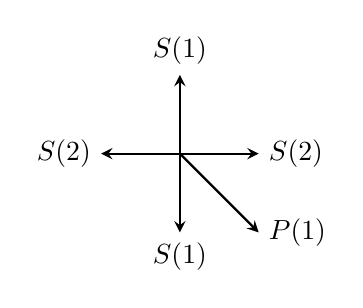
\begin{tikzpicture}[>=stealth,scale=1,line cap=round,
			bullet/.style={circle,inner sep=1.5pt,fill}]
			%\draw[->] (-5,0) -- (5,0) node[right]{$x$};
			%\draw[thick,->] (0,0) -- (1,-1) node[above][$L$]
			\draw[thick,->] (0,0) -- (1,0) node[right]{$S(2)$};
			\draw[thick,->] (0,0) -- (-1,0) node[left]{$S(2)$};
			\draw[thick,->] (0,0) -- (0,1) node[above]{$S(1)$};
			\draw[thick,->] (0,0) -- (0,-1) node[below]{$S(1)$};
			\draw[thick,->] (0,0) -- (1,-1) node[right]{$P(1)$};
			%\draw foreach \X in {3,6}
			%{(\X,0.1) -- ++ (0,-0.2) node[below]{$\X$}};
			%\draw foreach \Y in {2,4}
			%{(0.1,\Y) -- ++ (-0.2,0) node[left]{$\Y$}};
			
			%\foreach \X [count=\Y] in {(-1,0),(0,-1),(-2,1),(1,-3)} 
			%{\path  \X node(n\Y)[label=left:{$\X$}]{};
			%	\draw[dashed,->,opacity = 0.5]  (0,0) -- (n\Y);}
		\end{tikzpicture}
	\end{center}
	\caption{The walls of the path algebra $k\protect\overrightarrow{A_2}$.}
	\label{a2-walls}
\end{figure}

\subsection{Cones, walls and chambers induced by \tu-tilting pairs}
We now aim to recover information about the \tu-tilting theory of an algebra from its wall and chamber structure.

The following result hints to a connection between stability spaces and $\tu$-tilting theory.

\begin{theorem}\cite{auslander1985modules}[Theorem 1.4(a)]
	Let $M,N$ be modules. We have \[\langle g^M,[N]\rangle = hom_A(M,N) - hom_A(N,\tau M))\]
\end{theorem}


An important ingredient in this section will be the following formula, which follows from applying the above theorem twice.
\begin{proposition}[Corollary 3.10]\cite{Br_stle_2019}
	Let $(M,P)$ be a \tu-rigid pair. Then
 \[\langle g^{(M,P)},[N]\rangle = hom_A(M,N) - hom_A(N,\tau M) - hom_A(P,N)\]
\end{proposition}

\begin{proof}
	By \cite[Theorem 1.4(a)]{auslander1985modules}, we have $\langle g^M,[N]\rangle = hom_A(M,N) - hom_A(N,\tau M)$. Since $g^{(M,P)} = g^M - g^P$, we get
	\begin{align}
	&\langle g^{(M,P)},[N]\rangle \\
	=&\langle g^M,[N]\rangle - \langle g^P,[N]\rangle \\
	=&hom_A(M,N) - hom_A(N,\tau M) - hom_A(P,N) + hom_A(N,\tau P) \\
	=&hom_A(M,N) - hom_A(N,\tau M) - hom_A(P,N) + hom_A(N,0)\\
	=&hom_A(M,N) - hom_A(N,\tau M) -hom_A(P,N)
	\end{align}
\end{proof}

\comment{
Note that the above formula implies that a dimension vector $[X]$ with $X$ in a Jasso perpendicular $J(M,P) = J(M_1\oplus\dots\oplus M_i,P_1\oplus\dots\oplus P_j)$ will be orthogonal to $g^{(M,P)}$. Also, by additivity, $[X]$ will be orthogonal to any linear combination of the vectors $\{g^{M_1},\dots,g^{M_i},-g^{P_1},\dots,-g^{P_j}\}$. We now aim to prove a partial converse to this statement.}
\begin{definition}
	Let $T = (M,P)$ be a \tu-rigid pair. Following \cite{dij17}, we define the \textit{cone} spanned by $T$, as \[C(T) = \{\sum_{i = 1}^{j} \alpha_ig^{M_i} - \sum_{i = 1}^{k}\beta_ig^{P_i} : \alpha_i,\beta_i \geq 0 \text{ for all } i\}\]
	
	The interior $C^\circ(T) \subset C(T)$ is defined by requiring all coefficients $\alpha_i,\beta_i$ to be strictly positive.
\end{definition} 

Given a vector $\alpha = (\alpha_1,\alpha_2,\dots,\alpha_n)$ with $\alpha_i \geq 0$ for all $i$, we let $\alpha(M,P)$ denote the vector $G^{(M,P)} \times \alpha$.

\comment{

\begin{proposition}\cite{Br_stle_2019}[Proposition 3.13]
	For $\alpha(M,P) \in C^\circ(M,P)$, a module $N$ is $\alpha(M,P)$-semistable if and only if $N \in J(M,P)$.
\end{proposition}

Note that the simple objects in $J(M,P)$ are, by the proposition above, exactly the $\alpha(M,P)$-stable modules.
}

The cones $C(T)$ for support \tu-tilting pairs and almost complete support \tu-tilting pairs play an important role in the wall and chamber structure of an algebra. We summarize some of the most important results below.

\begin{proposition}\cite[Proposition 3.15, Corollary 3.16, Corollary 3.21]{Br_stle_2019}\label{tau-wall-chamber-result}, \cite[Theorem 3.17]{asai2020wallchamber}
	\begin{enumerate}
		\item For a support \tu-tilting pair $T_1 = (M,P)$, $C^\circ(T_1)$ defines a chamber in the wall and chamber structure of $A$.
		\item For an almost complete support \tu-tilting pair $T_2 = (M,P)$, $C(T_2)$ is included in a wall $\mathcal{D}(N)$ in the wall and chamber structure of $A$. The module $N$ may be computed given the two support \tu-tilting pairs containing $(M,P)$.
		\item All chambers are on the form $C^\circ(T)$ for a support \tu-tilting pair $T$.
		
	\end{enumerate}
\end{proposition}

The third point in the proposition above was first proved for \tu-tilting finite algebra in \cite{Br_stle_2019}, while Asai demonstrated the general case in \cite{asai2020wallchamber}.

The Kronecker algebra $K$, sometimes denoted $K_2$ in this thesis, supplies our most important example of wall and chamber structures. 

\begin{example}\label{limit-wall}
	Consider the Kronecker algebra $K$. Let $M$ be an indecomposable module with dimension vector $(1,1)$. Then $\mathcal{D}(M) = \{(x,-x):x \geq 0\}$. However, there is no \tu-rigid module with $g$-vector $(i,-i)$ for any $i \in \mathbb{N}$. This shows that not all walls come from (unions of) cones of almost complete support \tu-tilting pair.
\end{example}

We mow compute the wall and chamber structure of $K$, which will be references frequently in this thesis.

\begin{example}\label{k2-walls}
	Let $K$ be the Kronecker algebra. We wish to compute $g$-vectors of indecomposable $\tu$-rigid objects over $K$. Since $K$ has $2$ simple modules, these modules (together with $(0,P(1))$ and $(0,P(2))$) give the almost complete partial support $\tu$-tilting objects of $K$. 
	
	
	 $K$ has Cartan and Coxeter matrices given by \begin{align}
		C = \begin{bmatrix}
			1 & 0 \\ 2 & 1
		\end{bmatrix} && \Phi = \begin{bmatrix} -1 & 2 \\ -2 & 3\end{bmatrix}
	\end{align}
	
	It follows from \cite[Chapter 4, corollary 2.9)]{assem_skowronski_simson_2006} and \cite[Chapter 4, corollary 2.7)]{assem_skowronski_simson_2006} that the dimension vector of $\tau^{-i}P(i)$ is $\Phi^i\times \text{dim}(P(i))$ and that the dimension vector of $\tau^{i}I(i)$ is $\Phi^{-i}\times \text{dim}(I(i))$.
	
	Also, observe the minimal projective presentation of a module depends only on its dimension vector. A module over $K$ with dimension vector $d$ has $g$-vector $C^{-1}d$.
	
	Then any object in the postprojective component on the form $\tau^{-i}P(1)$ will have $g$-vector $(1+2i,-2i)$ and those on the form $\tau^{-i}P(2)$ will have $g$-vector $(2i,1-2i)$. Thus for all $j \in \mathbb{N}$ there is a postprojective module with $g$-vector on the form $(j+1,-j)$.
	
	Dually, the preinjective modules have $g$-vectors that are on the form $(j,-(j+1))$. The positive span of these $g$-vectors gives us subsets of walls in the wall and chamber structure of $K$, as guaranteed by \cref*{tau-wall-chamber-result}. For example, the $g$-vectors of $(P(1),0)$ and $(0,P(1))$ both lie in the wall $\mathcal{D}(S(2))$. 
	
	We claim that any wall $W$ is given as a union of rays in \cref{k2-wall-and-chamber}. To see this, observe that cones of the support $\tu$-tilting objects hit $\mathbb{R}^2$ minus the ray given by the positive span of $(1,-1)$. Since this ray in fact corresponds to a wall (the "limit wall"), any ray not drawn in the picture, which is also part of a wall must intersect a chamber, which is impossible.
	
	\begin{figure}[h]
		\begin{center}
			\begin{tikzpicture}[>=stealth,scale=1,line cap=round,
				bullet/.style={circle,inner sep=1.5pt,fill}]
				%\draw[->] (-5,0) -- (5,0) node[right]{$x$};
				%\draw[thick,->] (0,0) -- (1,-1) node[above][$L$]
				\draw[thick,->] (0,0) -- (1,-1) node[above]{$$};
				%\draw foreach \X in {3,6}
				%{(\X,0.1) -- ++ (0,-0.2) node[below]{$\X$}};
				%\draw foreach \Y in {2,4}
				%{(0.1,\Y) -- ++ (-0.2,0) node[left]{$\Y$}};
				\foreach \X [count=\Y] in {(1,0),(0,1),(2,-1),(3,-2),(1,-2),(2,-3),(-1,0),(0,-1),(-1,1)} 
				{\path  \X node(n\Y)[label=right:{$$}]{};
					\draw[dashed,->,opacity = 0.5]  (0,0) -- (n\Y);}
				
				%\foreach \X [count=\Y] in {(-1,0),(0,-1),(-2,1),(1,-3)} 
				%{\path  \X node(n\Y)[label=left:{$\X$}]{};
				%	\draw[dashed,->,opacity = 0.5]  (0,0) -- (n\Y);}
			\end{tikzpicture}
		\end{center}
		\caption{A finite portion of the walls of $K$, where the bold vector indicates the wall discussed in \cref{limit-wall}, appropriately called a limit wall.}
		\label{k2-wall-and-chamber}
	\end{figure}
	

\end{example}

The following reduction technique is very useful.

\begin{proposition}\cite[Lemma 4.13]{Br_stle_2019}\label{wall-reduction-quotient}
	Let $A$ be a finite dimensional algebra. Let $B = A/I$ be a quotient, where $I \subseteq \rad$. In particular, I  does not contain any non-trivial idempotents. There is then a canonical isomorphism between $K_0(A)$ and $K_0(B)$. Using this isomorphism, walls in the wall and chamber structure of $B$ are taken to walls in the wall and chamber structure of $A$.
\end{proposition}

\begin{proof}
	We have a canonical map $f:A \to A/I$. A module $M$ over $B$ may be considered an $A$-module, under the action $\alpha x = f(\alpha)x$. The important observation is now that the submodules of $M$ considered as an $A$-module coincide with the submodules of $M$ considered as a $B$-module.
	
	We prove one direction of this. Let $N \subset M$ be a $A$-submodule of $M$. We need to put a $B$-module structure on $N$. We attempt to define $f(\alpha)x = \alpha x$ for $\alpha \in A$ and prove that this is well-defined: $f(\alpha) = f(\beta)$ for some $\beta \in A$. Then $f(\alpha - \beta)x = 0$, so $\alpha-\beta \in I$. Thus $(\alpha-\beta)x = 0$, as $x \in M$. So the action is well-defined. The other direction is trivial.
	
	The rest of the proof now follows from the definition of a wall. See also the proof given in \cite{Br_stle_2019}.
\end{proof}

Using the third point of \cref{tau-wall-chamber-result}, we may conclude that an algebra with infinitely many walls in its wall and chamber structure will be \tu-tilting infinite. It is well known that algebras whose quivers have a double arrow are representation infinite. Here we show that they are \tu-tilting infinite as well.


\begin{proposition}
	Any algebra $A = k\Gamma/I$ where $\Gamma$ has a double arrow is \tu-tilting infinite.
\end{proposition}

\begin{proof}
	Choose a pair of double arrows. Let $J$ be the ideal generated by all arrows except the chosen pair of double arrows. Then $A/J$ decomposes as an algebra to $A/J = K_2 \times k \times k \times \dots \times k$. Since $K_2$ is $\tau$-tilting infinite, $A/J$ is also $\tau$-tilting infinite and must then have infinitely many walls.
	
	Thus by \cref{wall-reduction-quotient}, $A$ has infinitely many walls and is thus $\tau$-tilting infinite.
\end{proof}


\subsection{Consequences for the structure of $Q(s\tu\text{-tilt})$}


This following result shows that cones of $\tau$-rigid objects intersect in a very controlled fashion.

\begin{proposition}\cite[Corollary 6.7, b)]{dij17}
	Let $T_1,T_2$ be support \tu-tilting pairs. Then $C(T_1) \cap C(T_2) = C(X)$ with $X$ being the maximal \tu-rigid pair such that $X$ is a summand of $T_1$ and of $T_2$.
\end{proposition}

This result gives a tool for classifying all support \tu-tilting pairs. We collect this technique as a proposition.

\begin{proposition}\cite{dij17}
	Let $A$ be an algebra.
	
	\begin{itemize}
		\item If $A$ is \tu-tilting finite, its mutation graph is connected, thus the set of support \tu-tilting pairs over $A$ are exactly the ones in this component.
		\item If it is \tu-tilting infinite the mutation graph may be disconnected. Let $X$ be a set of support \tu-tilting pairs such that $\cup_{T \in X} C(T)$ is dense in $\mathbb{R}^n$. Then $X$ contains all support \tu-tilting pairs over $A$.
		
	\end{itemize}
\end{proposition}

\begin{proof}
	The \tu-tilting finite case is well-known.
	
	Let $T = (M,P)$ be a support \tu-tilting pair. Consider a point $x \in C(T)$ in the interior of $C(T)$. Since $\cup_{T \in X} C(T)$ is dense in $\mathbb{R}^n$, there is a $T_2$ in $X$ such that $C(T_2) \cap C(T)$ contains $x$. But $C(T_2)\cap C(T) = C(Y)$ for some partial support \tu-tilting pair $Y$. Since $T \neq T_2$, there is a summand $Z$ in $T = (M,P)$ not in $Y$. Writing $x$ as an element of $C(T)$, we get
	
	\[x = \sum_{i = 1}^{j} \alpha_ig^{M_i} - \sum_{i = 1}^{k}\beta_ig^{P_i}\]

	The above expression also gives a way of writing $x$ as an element of  $C(T)$, where in particular the $g^{Z}$ coordinates are $0$. Thus $x$ lies on the border of $C(T)$, giving us a contradiction.
	
\end{proof}

It is interesting to note that for tame algebras, the converse of the above theorem holds, in the sense that the closure of the union of all chambers must span $\mathbb{R}^n$, see \cite{keller2020tame}.

in \cite{dij17}, the authors use the above demonstrated criteria to classify the support \tu-tilting pairs of two specific symmetric algebras. We may however easily refine the criterion using ideas from\cite{Br_stle_2019}. We collect this refined technique as a theorem, which will be used frequently in this thesis.

\begin{theorem}\label{all_chambers_found}
	Let $A$ be an algebra. Let $W$ be the set of walls in the wall and chamber structure of $A$, and let $\overline{W}$ be its closure.
	
	Let $X$ be a set of support \tu-tilting pairs whose cones hit all chambers of $A$, i.e such that \[(\cup_{T \in X} C(T))  \cup \overline{W} = \mathbb{R}^n\]  then $X$ contains all support \tu-tilting pairs over $A$.
\end{theorem}

\begin{proof}
	The set of chambers $C$ in the wall and chamber structure of $A$ is defined as the connected components of $\mathbb{R}^n - \overline{W}$. If $(\cup_{T \in X} C(T))  \cup \overline{W} = \mathbb{R}^n$, then $\mathbb{R}^n - \overline{W} \subseteq (\cup_{T \in X} C(T))$. Thus every chamber $c \in C$ lies entirely inside $(\cup_{T \in X} C(T))$. Since chambers of different support \tu-tilting pairs only intersect on their boundary if they intersect at all, we may conclude that $c = C(T)$ for some $T \in X$. This finishes the proof.
\end{proof}


\subsection{Wall crossing and green sequences}
We can employ the wall and chamber structure to detect the non-existence of maximal green sequences. A maximal green sequence in $Q(s\tu\text{-tilt} A)$ is a path from $(A,0)$ to $(0,A)$ using only left mutations or equivalently respecting the orientation of the edges.

We will see that mutations in $Q(s\tu\text{-tilt} A)$ are closely linked to certain paths in the wall and chamber structure of $A$.

\begin{definition}\cite[Definition 4.1]{Br_stle_2019}%add citation
	A smooth path $\gamma:[0,1] \to \mathbb{R}^n$ is called a $\mathcal{D}$-generic path if:
	
	\begin{enumerate}
		\item Both $\gamma(0)$ and $\gamma(1)$ lie in the interior of some chamber.
		\item If $\gamma(t)$ lies in the intersection of two walls, the dimension vectors of the modules determining these walls must be scalar multiples of each other. Note that this means that $\gamma(t) \neq 0$ for all $t$.
		\item $\gamma(t) \in \mathcal{D}(M)$ implies $\langle \gamma'(t),[M]\rangle \neq 0$.
	\end{enumerate}

	Further, when $\gamma(t)$ lies in a wall $\mathcal{D}(M)$, we say that the crossing is \textit{green} if $\langle \gamma'(t),[M]\rangle > 0$ and red if $\langle \gamma'(t),[M]\rangle < 0$. A $\mathcal{D}$-generic path is then called green if all such crossings are green.
\end{definition}

In \cite[Lemma 4.2]{Br_stle_2019}, the authors construct explicitly a $\mathcal{D}$-generic path moving from the chamber of some support \tu-tilting pair $(M,P)$ to the chamber induced by a mutation of $(M,P)$, passing exactly one wall.

Inductively, they show in \cite[Theorem 4.3]{Br_stle_2019} that a sequence of left and right mutations from $(M_1,P_1)$ to $(M_2,P_2)$ induces a $\mathcal{D}$-generic path between $C^\circ(M_1,P_1)$ and $C^\circ(M_2,P_2)$ passing one wall for each mutation. The following corollary will be used later.

\begin{corollary}\label{corollary-dgeneric}
	Let $T = (M_1,P_1)$ and $T = (M_2,P_2)$ be support \tu-tilting pairs over $A$.
	
	If there is no $\mathcal{D}$-generic path $\gamma$ from $C^\circ(T_1)$ and $C^\circ(T_2)$ in the wall and chamber structure of $A$ passing only finitely many walls, then $T_1$ and $T_2$ lie in different components of $Q(s\tau\text{-tilt} A)$
\end{corollary}

\begin{proof}
	This is the contra-positive of the result discussed above; \cite[Theorem 4.3]{Br_stle_2019}.
\end{proof}

\section{Main results}
We now exploit the techniques discussed so far to determine properties of mutation quivers $Q(s\tau\text{-tilt} A)$ for various algebras $A$.


\subsection{Inheriting mutation from Kronecker algebras}
The idea of the following theorem is to use the \tu-tilting theory of the Kronecker algebra with two arrows, $K$, to explicitly compute mutations in a more complicated algebra.

\begin{theorem}\label{k2-reduction}
	Let $A$ be the algebra $kQ/r^2$ where $Q$ is the quiver	
	\[\begin{tikzcd}
	1 
	\arrow[r,bend left,shift right = 0.5ex, "\beta"]
	\arrow[r,bend left, shift left = 2ex, "\alpha"]
	& 2 \arrow[l,bend left,shift right = 0.5ex,"\gamma"]
	\arrow[l,bend left,shift left = 2ex, "\delta"]  \\
		\end{tikzcd}
	\]
	
	Then $Q(s\tau\text{-tilt } A)$ has exactly two components.
		
\end{theorem}



\begin{proof}
	A module $M$ over $A$ where either the maps induced by $\gamma$ and $\delta$, or $\alpha$ and $\beta$ are zero may naturally be considered a $K_2$-module.
	
	Then it is not difficult to see that the $g$-vector of such an $M$ as a $K_2$-module is the same as the $g$-vector of $M$ as an $A$-module, up to switching coordinates (if we demand that arrows go from vertex $1$ to $2$ in $K_2$, we need to do this swap for the case where $M$ is an $A$-module where $\alpha,\beta$ are zero).
	
	Consider the mutation of $P(1) \oplus P(2)$ at $P(1)$.
	
	\[P(1) \xrightarrow{\begin{bmatrix} \gamma \\ \delta\end{bmatrix}} P(2) \oplus P(2)\]
	
	Is a minimal left $P(2)$-approximation of $P(1)$, and its cokernel $X$ is naturally a $K$ module, as $\alpha X = 0$, and $\beta X= 0$. It is also $\tau$-rigid as a $K$ module. We thus have a \tu-tilting pair $T = (P(2)\oplus X,0)$ over $A$, which may naturally be considered a \tu-tilting pair over $K_2$. 
	
	This means that all iterated left mutations from $T$ are controlled by mutation in $K_2$. 
	
	A symmetrical argument shows that mutating $P(1) \oplus P(2)$ at $P(2)$ gives a \tu-tilting module whose iterated left-mutations are again dictated by mutation on $K_2$.
	
	Thus we may compute the $g$-vectors of these \tu-tilting modules, as shown in the figure.
	
	
		\begin{figure}[h]
			\begin{center}
			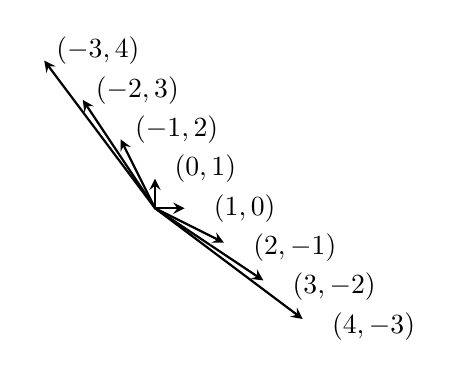
\begin{tikzpicture}[>=stealth,scale=0.5,line cap=round,
		bullet/.style={circle,inner sep=1.5pt,fill}]
		%\draw[->] (-5,0) -- (5,0) node[right]{$x$};
		%\draw[->] (0,-5) -- (0,5) node[above]{$y$};
		%\draw foreach \X in {3,6}
		%{(\X,0.1) -- ++ (0,-0.2) node[below]{$\X$}};
		%\draw foreach \Y in {2,4}
		%{(0.1,\Y) -- ++ (-0.2,0) node[left]{$\Y$}};
		\foreach \X [count=\Y] in {(1,0),(0,1),(-1,2),(-2,3),(-3,4),(2,-1),(3,-2),(4,-3)} 
		{\path  \X node(n\Y)[label=right:{$\X$}]{};
			\draw[thick,->]  (0,0) -- (n\Y);}
		\end{tikzpicture}
			\end{center}
		\caption{The $g$-vectors given by indecomposable summands of support \tu-tilting pairs at most three left mutations from $(P(1) \oplus P(2),0)$ for the algebra $A$}
		\end{figure}
	
	The closure of the cones coming from the support \tu-tilting pairs which are left mutations of $(P(1) \oplus P(2),0)$ clearly hit any point $(x,y) \in \mathbb{R}^2$ where $y + x \geq 0$. 
	
	By the duality on $g$-vectors discussed in \cref{duality-g-vector}, we  see that the closure of the cones coming from iterated right mutations of $(0,P(1)\oplus P(2))$ hit any point $(x,y) \in \mathbb{R}^2$ where $y + x \leq 0$. 
	
	Thus we see that every point $(x,y) \in \mathbb{R}^2$ lies in the closure of the cones coming from support \tu-tilting pairs in these two components. This concludes the proof.
	
	
\end{proof}

We may generalize the theorem above slightly. Recall that the generalized Kronecker algebra $K_i$ is the path algebra of the quiver with vertices $\{1,2\}$ and $i$ arrows from $1$ to $2$, and no other arrows.
\begin{corollary}
	Let $A_{i,j}$ be the algebra on the form $kQ/r^2$ where $Q$ is on the form
	\[\begin{tikzcd}
	1
	\arrow[r, shift right = -3.5ex, draw=none, "\raisebox{+2.5ex}{\vdots}" description]
	\arrow[r,bend left,shift right = 0.5ex, "\alpha_i"]
	\arrow[r,bend left, shift left = 4ex, "\alpha_1"]
	& 2 \arrow[l, shift left = 5.0ex, draw=none, "\raisebox{+2.5ex}{\vdots}" description]
	\arrow[l,bend left,shift right = 0.5ex,"\beta_j"]
	\arrow[l,bend left,shift left = 4.0ex, "\beta_1"]  \\
	\end{tikzcd}
	\]
	
	Then $Q(s\tu\text{-tilt} A_{i,j})$ has exactly two connected components for all $i,j \geq 2$.
	
\end{corollary}

\begin{proof}
Entirely equivalent to the case where $i = 2 = j$, we will still have that left mutations of $P(1) \oplus P(2)$  behave as if they were left mutations appearing in the Kronecker algebra case.

	\begin{figure}[h]
	\begin{center}
		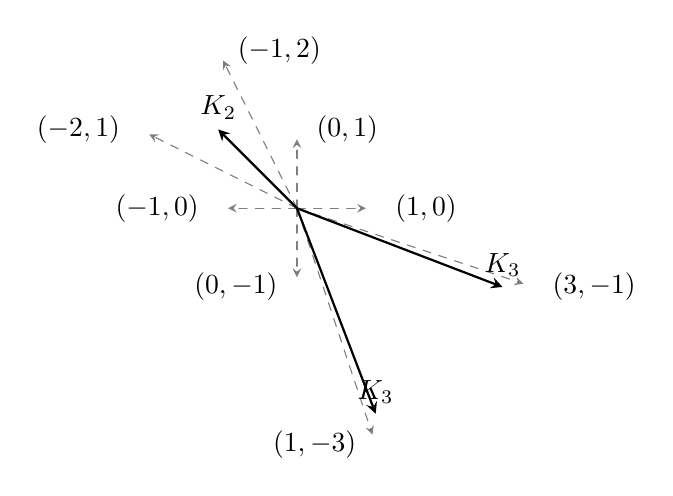
\begin{tikzpicture}[>=stealth,scale=1,line cap=round,
		bullet/.style={circle,inner sep=1.5pt,fill}]
		%\draw[->] (-5,0) -- (5,0) node[right]{$x$};
		\draw[thick,->] (0,0) -- (2.61,-1) node[above]{$K_3$};
		\draw[thick,->] (0,0) -- (1,-2.61) node[above]{$K_3$};
		\draw[thick,->] (0,0) -- (-1,1) node[above]{$K_2$};
		%\draw foreach \X in {3,6}
		%{(\X,0.1) -- ++ (0,-0.2) node[below]{$\X$}};
		%\draw foreach \Y in {2,4}
		%{(0.1,\Y) -- ++ (-0.2,0) node[left]{$\Y$}};
		\foreach \X [count=\Y] in {(1,0),(0,1),(-1,2),(3,-1)} 
		{\path  \X node(n\Y)[label=right:{$\X$}]{};
			\draw[dashed,->,opacity = 0.5]  (0,0) -- (n\Y);}
		
			\foreach \X [count=\Y] in {(-1,0),(0,-1),(-2,1),(1,-3)} 
		{\path  \X node(n\Y)[label=left:{$\X$}]{};
			\draw[dashed,->,opacity = 0.5]  (0,0) -- (n\Y);}
		\end{tikzpicture}
	\end{center}
	\caption{The $g$-vectors given by indecomposable summands of support \tu-tilting pairs at most two left mutations from $(P(1) \oplus P(2),0)$ or two right mutations from $(0,P(1)\oplus P(2))$ for the algebra $A_{3,2}$. The area between the vectors labeled $K_3$ is densely filled with walls.}
\end{figure}

The $g$-vectors of right mutations from $(0,P(1)\oplus P(2))$ may be computed indirectly by left mutations of $(P(1)^*\oplus P(2)^*,0)$ on $A^\text{op}$. 

Note that a wall $v$ in $K_i$  gives a wall $v$ in $A_{i,j}$. Also, a wall $w_1 = (x,y)$ in $K_j$ gives a wall $w_2 = (y,x)$ in $A_{i,j}$ because we need to swap the arrows in $K_j$ to view it as a quotient of $A_{i,j}$.

The closure cones of the identified support \tu-tilting pairs now span $\mathbb{R}^2 - C(W)$, were $C(W)$ is the closure of all walls. Thus by \cref{all_chambers_found}, these are all support \tu-tilting pairs.


\end{proof}

The following corollary gives an example of an algebra with more than two components in its \tu-tilting mutation quiver.

\begin{corollary}\label{4components}
	Let $A$ be the algebra on the form $kQ/r^2$ with the quiver.
	
	% https://q.uiver.app/?q=WzAsNCxbMCwwLCJcXGJ1bGxldCJdLFswLDEsIlxcYnVsbGV0Il0sWzIsMCwiXFxidWxsZXQiXSxbMiwxLCJcXGJ1bGxldCJdLFswLDEsIiIsMix7ImN1cnZlIjoxfV0sWzAsMSwiIiwwLHsiY3VydmUiOjJ9XSxbMSwwLCIiLDEseyJjdXJ2ZSI6MX1dLFsxLDAsIiIsMSx7ImN1cnZlIjoyfV0sWzIsMywiIiwxLHsiY3VydmUiOjF9XSxbMiwzLCIiLDEseyJjdXJ2ZSI6Mn1dLFszLDIsIiIsMSx7ImN1cnZlIjoxfV0sWzMsMiwiIiwxLHsiY3VydmUiOjJ9XSxbMCwyXV0=
	\[\begin{tikzcd}
	1 && 3 \\
	2 && 4
	\arrow[curve={height= 6pt}, from=1-1, to=2-1]
	\arrow[curve={height=12pt}, from=1-1, to=2-1]
	\arrow[curve={height=6pt}, from=2-1, to=1-1]
	\arrow[curve={height=12pt}, from=2-1, to=1-1]
	\arrow[curve={height=6pt}, from=1-3, to=2-3]
	\arrow[curve={height=12pt}, from=1-3, to=2-3]
	\arrow[curve={height=6pt}, from=2-3, to=1-3]
	\arrow[curve={height=12pt}, from=2-3, to=1-3]
	%\arrow[from=1-1, to=1-3]
	\end{tikzcd}\]
	
	Then $Q(s\tau\text{-tilt} A)$ has exactly $4$ connected components.
\end{corollary}

\begin{proof}
	Let $A_1 = P(1) \oplus P(2)$, $A_2 = P(3) \oplus P(4)$. Let $Q = Q(s\tu\text{-tilt} A)$.
	
	Then $Q(s\tu\text{-tilt} A)$ is, as a directed graph, the cartesian product of $Q(s\tu\text{-tilt} \text{End}(A_1))$ and $Q(s\tu\text{-tilt} \text{End}(A_2))$. Each of these have two connected components, so its product has four.
	
	More concretely, it is not hard to see that every support \tu-tilting pair must lie in the same components as either $(A_1\oplus A_2,0)$, $(A_1,A_2)$, $(A_2,A_1)$ or $(0,A_1 \oplus A_2)$ and that none of these four objects lie in the same component.
\end{proof}

We now discuss one consequence of the above result. It is natural to seek an algorithm which enumerates all support \tu-tilting pairs. For $\tu$-tilting finite algebras, the mutation quiver is connected, and may thus easily be traversed. More generally, for an algebra $A$ where every support \tu-tilting pair may be found in the same component as $(A,0)$ or $(0,A)$, one may enumerate all support $\tu$-tilting objects by recursively left- and right-mutating at $(A,0)$ and at $(0,A)$. The above corollary demonstrates that this algorithm does not in general enumerate all support \tu-tilting pairs.

There are also connected algebras with more than two components in its \tu-tilting mutation quiver.

\begin{corollary}
	Let $A$ be the algebra on the form $kQ/r^2$ with $Q$ as the quiver below.
	
	% https://q.uiver.app/?q=WzAsNCxbMCwwLCJcXGJ1bGxldCJdLFswLDEsIlxcYnVsbGV0Il0sWzIsMCwiXFxidWxsZXQiXSxbMiwxLCJcXGJ1bGxldCJdLFswLDEsIiIsMix7ImN1cnZlIjoxfV0sWzAsMSwiIiwwLHsiY3VydmUiOjJ9XSxbMSwwLCIiLDEseyJjdXJ2ZSI6MX1dLFsxLDAsIiIsMSx7ImN1cnZlIjoyfV0sWzIsMywiIiwxLHsiY3VydmUiOjF9XSxbMiwzLCIiLDEseyJjdXJ2ZSI6Mn1dLFszLDIsIiIsMSx7ImN1cnZlIjoxfV0sWzMsMiwiIiwxLHsiY3VydmUiOjJ9XSxbMCwyXV0=
	\[\begin{tikzcd}
	1 && 3 \\
	2 && 4
	\arrow[curve={height= 6pt}, from=1-1, to=2-1]
	\arrow[curve={height=12pt}, from=1-1, to=2-1]
	\arrow[curve={height=6pt}, from=2-1, to=1-1]
	\arrow[curve={height=12pt}, from=2-1, to=1-1]
	\arrow[curve={height=6pt}, from=1-3, to=2-3]
	\arrow[curve={height=12pt}, from=1-3, to=2-3]
	\arrow[curve={height=6pt}, from=2-3, to=1-3]
	\arrow[curve={height=12pt}, from=2-3, to=1-3]
	\arrow[from=1-1, to=1-3]
	\end{tikzcd}\]
	
	Then $Q(s\tau\text{-tilt} A)$ has at least $4$ connected components.
\end{corollary}


\begin{proof}
	
	 Note that $\text{Hom}_A(P(1)\oplus P(2),P(3)\oplus P(4)) = 0$ as there are no paths from vertices $3,4$ to vertices $1,2$. Thus \[T_1 = (P(3) \oplus P(4), P(1) \oplus P(2))\] is a support \tu-tilting pair. We intend now to show that it may not lie within a finite number of right or left mutations from $(A,0)$ and $(0,A)$. This means that $T_1$ must lie in a third component of $Q(s\tu\text{-tilt} A)$, as wanted.
	
	From \cite{Br_stle_2019}[Lemma 4.13], we see that a wall in the wall and chamber structure of the algebra presented in \cref{4components} gives a wall in the wall and chamber structure of $A$. Let $B$ be the algebra in \cref{4components}.
	
	Consider $T_{B,1} = ((P_B(3) \oplus P_B(4), P_B(1) \oplus P_B(2)))$. Then $T_{B,1}$ and $T_1$ will have equal $G$-matrices.
	
	\[G^{T_1} = \begin{bmatrix}
		0 & 0 & -1 & 0 \\ 0 & 0 & 0 & -1 \\ 1 & 0 & 0 & 0 \\ 0 & 1 & 0 & 0
	\end{bmatrix} = G^{T_{B,1}}\]
	
	This means in particular that $g^{T_1}$ lies in the cone of $T_{B,1}$. Assume now, that there is a $\mathcal{D}$-generic path $\gamma$ from $g^{T_1}$ to $g^{(A,0)} = (1,1,1,1)$ in $Q(s\tu\text{-tilt } A)$. In the wall and chamber structure of $B$, this path is also $\mathcal{D}$-generic and must cross infinitely may walls since $(B,0)$ and $T_{B,1}$ lie in different components of $Q(s\tau\text{-tilt} B)$. Now, since walls in $B$ induce walls in $A$, $\gamma$ must pass infinitely many walls also in $A$. 
	
	Then by \cref{corollary-dgeneric}, $T_1$ does not lie in the same component as $(A,0)$. A similar argument shows that it may not lie in the same component as $(0,A)$.
	
	To identify a fourth component, observe first that $(P(1)\oplus P(2),P(3)\oplus P(4))$ is not support \tu-tilting, as there is a nonzero map $P(3) \to P(1)$ induced by the path of length $1$ from $1$ to $3$. We consider instead the mutation $\mu_{P(1)}(P(1)\oplus P(2)\oplus P(3)\oplus P(4))$.
	
	Since $\text{Hom}(P(1),P(4)) = 0 = \text{Hom}_A(P(1),P(3))$, the mutation may be computed as a co-kernel of $P(2) \oplus P(2)$ exactly as in \cref{k2-reduction}.
	
	Let then \[X \oplus P(2) \oplus P(3) \oplus P(4) = \mu_{P(1)}(P(1)\oplus P(2) \oplus P(3)\oplus P(4))\]  $X$ can easily be computed to be a module with dimension vector $(3,2,0,0)$ and $g$-vector $(-1,2,0,0)$. 
	
	Since $\text{Hom}_A(P(3)\oplus P(4),X\oplus P(2)) = 0$ we get that \[T_2 = (X \oplus P(2), P(3) \oplus P(4))\] is a support \tu-tilting pair. Consider $T_{B,2} = \mu_{P_B(1)}((P_B(1) \oplus P_B(2), P_B(3) \oplus P_B(4)))$. Then $T_{B,2}$ and $T_2$ will have equal $G$-matrices.
	
	\[G^{T_2} = \begin{bmatrix}
		-1 & 0 & 0 & 0 \\ 2 & 1 & 0 & 0 \\ 0 & 0 & -1 & 0 \\ 0 & 0 & 0 & -1
	\end{bmatrix} = G^{T_{B,2}}\]
	
	This means in particular that $g^{T_2}$ lies in the cone of $T_{B,2}$. Again then we conclude that $T_2$ can not lie in the component containing $(A,0)$ or the component containing $(0,A)$. 
	
	Lastly, $T_2$ and $T_1$ themselves must also lie in two distinct components of $Q(s\tau\text{-tilt } A)$, because their $g$-vectors lie in cones corresponding to support $\tu$-tilting objects of $B$ lying in distinct components.
	
	This concludes our proof.
\end{proof}

\comment{
\begin{proof}
	Consider the mutation $\mu_{P(1)}(P(1)\oplus P(2)\oplus P(3)\oplus P(4))$.
	
	Since $\text{Hom}(P(1),P(4)) = 0 = \text{Hom}_A(P(1),P(3))$, the mutation may be computed as a co-kernel of $P(2) \oplus P(2)$ exactly as in \cref{k2-reduction}.
	
	Let then \[X \oplus P(2) \oplus P(3) \oplus P(4) = \mu_{P(1)}(P(1)\oplus P(2),P(3)\oplus P(4))\]  $X$ has dimension vector $(3,2,0,0)$ with $g$-vector $(-1,2,0,0)$. 
	
	Since $\text{Hom}_A(P(3)\oplus P(4),X\oplus P(2)) = 0$ we get that \[T = (X \oplus P(2), P(3) \oplus P(4))\] is a support \tu-tilting pair. We intend now to show that it may not lie within a finite number of right or left mutations from $(A,0)$ and from $(0,A)$. This means that $T$ must lie in a third component of $Q(s\tu\text{-tilt} A)$, as wanted.
	
	From \cite{Br_stle_2019}[Lemma 4.13], we see that a wall in the wall and chamber structure of the algebra presented in \cref{4components} gives a wall in the wall and chamber structure of $A$. Let $B$ be the algebra in \cref{4components}.
	
	Consider $T_B = \mu_{P_B(1)}((P_B(1) \oplus P_B(2), P_B(3) \oplus P_B(4)))$. Then $T_B$ and $T$ will have equal $G$-matrices.
	
	\[G^T = \begin{bmatrix}
		-1 & 0 & 0 & 0 \\ 2 & 1 & 0 & 0 \\ 0 & 0 & -1 & 0 \\ 0 & 0 & 0 & -1
	\end{bmatrix} = G^{T_B}\]
	
	This means in particular that $g^T$ lies in the cone of $T_B$. Assume now, that there is a $\mathcal{D}$-generic path $\gamma$ from $g^T$ to $g^{(A,0)} = (1,1,1,1)$ in $Q(s\tu\text{-tilt } A)$. In the wall and chamber structure of $B$, this path is also $\mathcal{D}$-generic and must cross infinitely may walls since $(B,0)$ and $T_B$ lie in different components of $Q(s\tau\text{-tilt} B)$. Now, since walls in $B$ induce walls in $A$, $\gamma$ must pass infinitely many walls also in $A$. 
	
	Then by \cref{corollary-dgeneric}, $T$ does not lie in the same component as $(A,0)$. A similar argument shows that it may not lie in the same component as $(0,A)$.
	
\end{proof}
}

\subsection{Inheriting $\tu$-rigid modules from $K_2$}
We will here further generalize \cref{k2-reduction}. Note that if we wish to study the algebra $A = kQ/r^3$ with $Q$ being the quiver

\[\begin{tikzcd}
	1 
	\arrow[r,bend left,shift right = 0.5ex, "\beta"]
	\arrow[r,bend left, shift left = 2ex, "\alpha"]
	& 2 \arrow[l,bend left,shift right = 0.5ex,"\gamma"]
	\arrow[l,bend left,shift left = 2ex, "\delta"]  \\
\end{tikzcd}
\]
we can no longer use the same proof as for \cref{k2-reduction} to compute its mutation quiver. In this section, we will show that we can us a different reduction from $K_2$ to compute $Q(s\tu\text{-tilt} A)$.


\begin{lemma}\label{2term-reduction}
	Let $A$ be an admissible quotient over some path algebra with a given ordering of its vertices, such that $\text{Hom}(P(2),P(1))$ is $2$-dimensional as a $k$-vector space. 
	
	\begin{enumerate}
		\item For any non-negative integer $n$ there is a $2$-term presilting complex in $K^b(\text{add} A)$, called $\mathbb{P}_A(n)$, on the form \[P(2)^n \to P(1)^{n+1}\]
		\item $\mathbb{P}_A(n) \oplus \mathbb{P}_A(n+1)$ is $2$-term presilting.
	\end{enumerate}
	
	In this case, we denote by $T_i$ the zeroth homology of $\mathbb{P}_A(i)$.
	

\end{lemma}

\begin{proof}
	(1.) The case where $n = 0$ is trivial, so assume that $n \geq 1$. Let first $K$ be the Kronecker algebra with two arrows. Let now $\mathbb{P}_K(n) $ be the unique indecomposable 2-term presilting object on the form \[P_K(2)^n \xrightarrow{f} P_K(1)^{n+1}\] over $K^b(\text{add} K)$. Note that $f$ may be viewed as an $n\times(n+1)$ matrix over $\text{Hom}_K(P(2),P(1))$ which is $2$-dimensional. Pick an isomorphism $\phi$ between $\text{Hom}_K(P(2),P(1))$ and $\text{Hom}_A(P(2),P(1))$. Then we may let $\phi$ act entry-wise on $f$. Call this induced map $\phi(f)$. We may also consider $\phi^{-1}$, which will have the symmetric property. We claim now that the complex $\mathbb{P}_A$ given by  \[P_A(2)^n \xrightarrow{\phi(f)} P_A(1)^{n+1}\] is rigid.
	
	% https://q.uiver.app/?q=WzAsNCxbMSwwLCJcXGJ1bGxldCJdLFsyLDAsIlxcYnVsbGV0Il0sWzAsMSwiXFxidWxsZXQiXSxbMSwxLCJcXGJ1bGxldCJdLFswLDFdLFsyLDNdLFswLDNdLFswLDJdLFsxLDNdXQ==

	To check rigidity of $\mathbb{P}_A$, we must show that $\text{Hom}_{K^b(\text{add} A)}(\mathbb{P}_A,\mathbb{P}_A[1]) = 0$, meaning that all maps from $\mathbb{P}_A$ to $\mathbb{P}_A$ shifted should be null-homotopic. Thus, we seek for any $g:P_A(2)^n \to P_A(1)^{n+1}$ two maps $h^A_1$ and $h^A_2$, such that $\phi(f)\circ h^A_1 + h^A_2 \circ \phi(f) = g$. This setup is drawn below.
	
	% https://tikzcd.yichuanshen.de/#N4Igdg9gJgpgziAXAbVABwnAlgFyxMJZARgBoAGAXVJADcBDAGwFcYkQAFAfQEEAKAEwBKAHqEAvqXSZc+QigEVqdJq3bd+xUcDABqYuJCTp2PASLlSxZQxZtEnXoNESpIDKblEy1mrbUOGnxaIjr6huLKMFAA5vBEoABmAE4QALZIliA4EEgAzH6q9iAxRm4p6Zk0OUhkKnbsADqNaAAWWHyJQmVJqRmIitm5iAX1ASDNbR1dPSAV-Vk1AzSMWGDFUBA4ONEghQ0OrVzEIjx7IIz0AEYwjBwyZvIgyVgxrTiz87XVw6Or6+xNttdvtxkcBKcjJRxEA
	\[\begin{tikzcd}
		& P_A(2)^n \arrow[d, "g"] \arrow[r, "\phi(f)"] \arrow[ld, "h_1^A"', dotted] & P_A(1)^{n+1} \arrow[ld, "h_2^A", dotted] \\
		P_A(2)^n \arrow[r, "\phi(f)"] & P_A(1)^{n+1}                                                              &                                         
	\end{tikzcd}
	\]
	
	 Certainly, $\phi^{-1}(g)$ is well-defined. Since \[P_K(2)^n \xrightarrow{f} P_K(1)^{n+1}\] is rigid, given the map $\phi^{-1}(g)$, there are maps $h_1:P_K(2)^n \to P_K(2)^n$ and $h_2:P_K(1)^{n+1} \to P_K(1)^{n+1}$ such that $h_2\circ f + f \circ h_1 = \phi^{-1}(g)$. This setup is drawn below.
	 
	\[
	% https://tikzcd.yichuanshen.de/#N4Igdg9gJgpgziAXAbVABwnAlgFyxMJZARgBoAGAXVJADcBDAGwFcYkQAFAfQGkAKAEwBKAHqEAvqXSZc+QigEVqdJq3bd+xUcDABqYuJCTp2PASLlSxZQxZtEnXoNESpIDKblEy1mrbUOGnxaIjr6huLKMFAA5vBEoABmAE4QALZIliA4EEgAzH6q9iAAOiVoABZYoQC0BnwxQkZuKemZNDlIZCp27InNSakZiIrZuYgFPQGl5VV8iU3GIK3DWZ0jNIxYYMVQEDg40SCFvQ4VXMTHIIz0AEYwjBwyZvIgyVgxFTgDy0NdHeNJlsduw9gcjidpucBEZKOIgA
	\begin{tikzcd}
		& P_K(2)^n \arrow[d, "\phi^{-1}(g)"] \arrow[r, "f"] \arrow[ld, "h_1"', dotted] & P_K(1)^{n+1} \arrow[ld, "h_2", dotted] \\
		P_K(2)^n \arrow[r, "\phi(f)"] & P_K(1)^{n+1}                                                                 &                                       
	\end{tikzcd}
	\] 
	
	 Note that $h_1$ and $h_2$ are scalar matrices, and may thus also be considered elements of $\text{End}_A(P_A(2))$ and $\text{End}_A(P_A(1))$ respectively. We may conclude that $\phi(h_2\circ f + f \circ h_1) = g$. The left hand side might be computed to be $h_2 \circ \phi(f) + \phi(f) \circ h_1$. We then have the equality $h_2 \circ \phi(f) + \phi(f) \circ h_1 = g$ as wanted. Letting $h^A_1 = h_1$ and $h^A_2 = h_2$, we conclude the proof.
	
	2. Let $\mathbb{T}_K = \mathbb{P}_K(n) \oplus \mathbb{P}_K(n+1)$. Then $\mathbb{T}_K$ is $2$-term pre-silting. We may then apply essentially the same proof as for (1.) to see that the corresponding $\mathbb{T}_A = \mathbb{P}_A(n) \oplus \mathbb{P}_A(n+1)$ must be rigid.
	
\end{proof}

We give two examples utilizing this lemma.

\begin{example}
	Consider the algebra $A = kQ/r^3$, where $Q$ is the quiver below.
	% https://q.uiver.app/?q=WzAsNCxbMCwxLCIxIl0sWzEsMCwiNCJdLFsxLDIsIlxcYnVsbGV0Il0sWzIsMSwiMiJdLFswLDFdLFswLDJdLFsyLDNdLFsxLDNdLFsxLDJdXQ==
	\[\begin{tikzcd}
		& 3 \\
		1 && 2 \\
		& 4
		\arrow[from=2-1, to=1-2]
		\arrow[from=2-1, to=3-2]
		\arrow[from=3-2, to=2-3]
		\arrow[from=1-2, to=2-3]
		\arrow[from=1-2, to=3-2]
	\end{tikzcd}\]

	Of course, in $kQ$, there are three paths from $1$ to $2$. However, the path of length $3$ is eliminated in the quotient $A$. Since the paths $1 \to 3 \to 2$ and $1 \to 4 \to 2$ are not identified in $A$, we may conclude that $\text{Hom}_A(P(2),P(1))$ is $2$-dimensional. We may now employ GAP to compute $\mathbb{P}_A(1)$. The zeroth homology of this complex gives us a module,say $T_1$, (with dimensions as displayed below). This module must be \tu-rigid from \cref{2term-reduction}, which we may be confirmed using GAP. In this case, the module is also indecomposable.
	\[\begin{tikzcd}
		& k^2 \\
		k^2 && k^3 \\
		& k^4
		\arrow[from=2-1, to=1-2]
		\arrow[from=2-1, to=3-2]
		\arrow[from=3-2, to=2-3]
		\arrow[from=1-2, to=2-3]
		\arrow[from=1-2, to=3-2]
	\end{tikzcd}\]


\end{example}

\begin{example}\label{example-decomposing-modules}
	Let $A = kQ/\beta^2$ where $Q$ is the quiver below.
	
	\[
	\begin{tikzcd}
		1 & 2
		\arrow[from=1-1,to=1-2,"\alpha"]
		\arrow[loop,from = 1-2,to=1-2,"\beta"',distance=2em]
	\end{tikzcd}
	\]
	
	This algebra is $\tu$-tilting finite, and $\text{Hom}_A(P(2),P(1))$ is $2$-dimensional. We are still promised an infinite family of $\tu$-tilting objects from \cref{2term-reduction}, where we let $T_i$ be as in the lemma. The consequence must be that almost all modules coming from this lemma must decompose. To investigate this, we first compute $Q(s\tau\text{-tilt} A)$. The mutation quiver is displayed in \cref{mutation-quiver-example-decomposing-modules}, where the vertices are written as support \tu-tilting pairs.
	
	% https://q.uiver.app/?q=WzAsNixbMSwwLCIoUCgxKVxcb3BsdXMgUCgyKSwwKSJdLFswLDEsIihQKDIpLFAoMSkpIl0sWzIsMSwiKFAoMSkgXFxvcGx1cyBUKDEpKSwwKSJdLFsyLDIsIihTKDEpXFxvcGx1cyBUKDEpLDApIl0sWzIsMywiKFMoMSksUCgyKSkiXSxbMSw0LCIoMCxQKDEpXFxvcGx1cyBQKDIpKSJdLFswLDFdLFswLDJdLFsyLDNdLFszLDRdLFs0LDVdLFsxLDVdXQ==
	\begin{figure}[h]
		\[\begin{tikzcd}
		& {(P(1)\oplus P(2),0)} \\
		{(P(2),P(1))} && {(P(1) \oplus T_1,0)} \\
		&& {(S(1)\oplus T_1,0)} \\
		&& {(S(1),P(2))} \\
		& {(0,P(1)\oplus P(2))}
		\arrow[from=1-2, to=2-1]
		\arrow[from=1-2, to=2-3]
		\arrow[from=2-3, to=3-3]
		\arrow[from=3-3, to=4-3]
		\arrow[from=4-3, to=5-2]
		\arrow[from=2-1, to=5-2]
	\end{tikzcd}\]
\caption{The mutation quiver of $A$ from \cref{example-decomposing-modules}.}
\label{mutation-quiver-example-decomposing-modules}
	\end{figure}

	
	$T_0 = P(1)$ and is thus clearly indecomposable. $T_1$ shows up as a summand in the mutation quiver and is indecomposable. Since any \tu-rigid module must show up in the mutation quiver as a summand of some support \tu-tilting pair, all $T_i$ for $i > 1$ must decompose into other \tu-rigid objects. We know that \tu-rigid modules are uniquely identified by their $g$-vectors. We also know that $S(1)$ has $g$-vector $(1,-1)$, and that $S(1) \oplus T_1$ is \tu-rigid. Thus we have the following equation 
	\[g^{T_i} = (i+1,-i) = g^{T_1^{i-1} \oplus S(1)}\]
	
	Thus it follows that in fact $T_i \cong T_1^{i-1} \oplus S(1)$ for all $i > 1$.
\end{example}

The above example shows that to fully utilize \cref{2term-reduction}, we need a criterion for indecomposability of the modules produced by the lemma. 

In the next lemma, we give an elementary example of such a condition for the case where $A$ has two simple modules. We dare hope that there exists a similar criterion which may be applied for algebras with more than two simple modules, but for our purposes the following tool will be sufficient.

\begin{lemma}\label{2-simple-criterion-T_i}
	Let $A$ be as in \cref{2term-reduction}, where $A$ has two simple modules. Assume that $(1,-1)$ is not a $g$-vector of $A$.	
	
	Then $T_i$ is indecomposable for all $i \geq 0$.
\end{lemma}

\begin{proof}
	 By the second part of \cref{2term-reduction}, we know that $T_k \oplus T_{k+1}$ is $\tu$-rigid for all $k \geq 0$.
	 
	 To seek a contradiction, assume that $k \geq 1$ is the smallest integer such that $T_k$ decomposes ($T_0$ is projective indecomposable). Recall that the $g$-vector of $T_i$ is $(i+1,-i)$, and that a basic \tu-rigid module over $A$ may have at most two summands.
	 
	 $A$ has $2$ simple modules, so any basic $\tu$-tilting object must have at most $2$ summands.  If $T_k$ decomposes, $T_{k-1} \oplus T_k$ has at least three summands, and must therefore not be basic. Since $T_{k-1}$ is indecomposable, this means that $T_k$ must decompose in one of the following ways.
	 
	 \begin{enumerate}
	 	\item $T_k \cong X^n$, where $n \geq 2$.
	 	\item $T_k = T_{k-1} \oplus Y$ 
	 	
	 \end{enumerate} 
	 
	 Indeed, if $T_k$ decomposes into an object with at least two non-isomorphic summands, then one of them must be isomorphic to $T_{k-1}$. Otherwise the sum $T_{k-1} \oplus T_k$ could not be \tu-rigid.
	 	 
	 The first case is not possible, because $-k$ and $k+1$ are relatively prime; thus $g^{T_k} = (k+1,-k)$ cannot be written as $m v$ for some other $g$-vector $v$ and integer $m > 1$. In the second case, $Y$ would be $\tu$-rigid with $g$-vector $(1,-1)$ by additivity, contradicting our assumptions. 
\end{proof}

We may now work with a class of algebras including the one mentioned in the introduction to this section.

\begin{theorem}\label{kq/r3}
	Let $A = kQ/I$ be an algebra where $Q$ is as  below and $I$ is an admissible ideal with $r^3 \subseteq I$. Then $Q(s\tu\text{-tilt} A)$ has exactly two components.
	\[\begin{tikzcd}
		1 
		\arrow[r,bend left,shift right = 0.5ex, "\beta"]
		\arrow[r,bend left, shift left = 2ex, "\alpha"]
		& 2 \arrow[l,bend left,shift right = 0.5ex,"\gamma"]
		\arrow[l,bend left,shift left = 2ex, "\delta"]  \\
	\end{tikzcd}
	\]
\end{theorem}

\begin{proof}
	First, note that for any choice of $I$ as given above, paths of length $3$ are killed in the quotient $kQ/I$, so $\text{Hom}(P(1),P(2))$ and $\text{Hom}(P(2),P(1))$ are both $2$-dimensional as $k$-vector spaces. We may thus apply \cref{2term-reduction} and the dual version of it. 
	
	Let $T_i$ be the \tu-rigid module with $g$-vector $(i+1,-i)$ coming from \cref{2term-reduction}. We wish to apply \cref{2-simple-criterion-T_i}.
	
	We need to show that $(1,-1)$ may not be a $g$-vector of any partial \tu-tilting module over $A$. 
	
	Observe that any open neighborhood around the point $(1,-1)$ as a point in $\mathbb{R}^2$ intersects infinitely many walls in the wall and chamber structure of $A$ (see \cref{walls-k2-k2}). Thus $(1,-1)$ cannot be lie inside a chamber. Also, given any $v \neq 0$ not parallel to  $(1,-1)$, we see that there exists for any real $\epsilon > 0$ an $\alpha < \epsilon$ such that $(1,-1) + \alpha v$ crosses a wall. Thus there cannot exist a chamber having $(1,-1)$ as a wall.
	
	We have thus infinitely many chambers on the form $C(T_i\oplus T_{i+1})$ for $i \geq 0$. Using the fact that $\text{Hom}(P(1),P(2))$ and $\text{Hom}(P(2),P(1))$ are both $2$-dimensional, we see that the closure of the chambers of the component of $Q(s\tu\text{-tilt} A)$ containing $(P(1)\oplus P(2),0)$ contains all points $(x,y) \in \mathbb{R}^2$ where $x+y \geq 0$. Dually, since $A^{\text{op}}$ satisfies the same assumptions as we needed about $A$, the closure of the chambers of the component containing $(0,P(1)\oplus P(2))$ must contain all points $(x,y)$ where $x + y\leq 0$.
	
	We may then conclude that $Q(s\tu\text{-tilt} A)$ has exactly two components in its mutation quiver.
	
		\begin{figure}[h]
		\begin{center}
			\begin{tikzpicture}[>=stealth,scale=1,line cap=round,
				bullet/.style={circle,inner sep=1.5pt,fill}]
				%\draw[->] (-5,0) -- (5,0) node[right]{$x$};
				\draw[thick,->] (0,0) -- (-1,1) node[above]{};
				\draw[thick,->] (0,0) -- (1,-1) node[above]{};
				%\draw foreach \X in {3,6}
				%{(\X,0.1) -- ++ (0,-0.2) node[below]{$\X$}};
				%\draw foreach \Y in {2,4}
				%{(0.1,\Y) -- ++ (-0.2,0) node[left]{$\Y$}};
				\foreach \X [count=\Y] in {(1,0),(0,1),(-1,2),(-2,3),(2,-1),(3,-2),(4,-3),(-3,4)} 
				{\path  \X node(n\Y)[label=right:{}]{};
					\draw[dashed,->,opacity = 0.3]  (0,0) -- (n\Y);}
				
				\foreach \X [count=\Y] in {(-1,0),(0,-1),(1,-2),(2,-3),(-2,1),(-3,2),(3,-4),(-4,3)} 
				{\path  \X node(n\Y)[label=left:{}]{};
					\draw[dashed,->,opacity = 0.3]  (0,0) -- (n\Y);}
			\end{tikzpicture}
		\end{center}
		\caption{Some of the walls inherited from $K_2$ in two different ways into $A$. The bold arrows are contained in the closure of these walls, and point in directions $(1,-1)$ and $(-1,1)$.}
		\label{walls-k2-k2}
	\end{figure}
	
	
\end{proof}

\subsection{Reduction by homotopy equivalence}
The main idea needed to prove \cref{kq/r3} is that the $2$-term silting objects of $K_2$ can say something about $2$-term silting objects over richer module categories. However, the proof above also requires some non-trivial technicalities because the category of $2$-term objects of projective $K_2$-modules are not equivalent to the category of $2$-term objects of projective modules in the more complicated category.

In the setting where we require this to hold, stronger reduction results hold.

\begin{proposition}\label{silting-equivalence}
	Let $A$ be an algebra, and let $P = \bigoplus_{i \in I} P(k)$ be the direct sum of indecomposable projective modules. Let $B$ be an algebra such that $\text{add } B \cong \text{add } P$ holds. Then
	\[K^b(\text{add } B) \cong K^b(\text{add } P)\]
	
	and there is a bijection between indecomposable $2$-term pre-silting complexes over $B$ and indecomposable $2$-term pre-silting objects over $A$ having $g$-vectors with support on $I$.
\end{proposition}

\begin{proof}
	 The proposition follows immediately from noting that $K^b(\text{add } P)$ embeds naturally into $K^b(\text{add } A)$, where the $2$-term silting complexes over $A$ live.
\end{proof}

\begin{proposition}
	Let $Q$ be an acyclic quiver, and let $A = kQ/I$ with $I$ an admissible ideal. If there exists indecomposable projective modules $P$ and $Q$ such that $\text{Hom}_A(Q,P)$ is $i$-dimensional as a $k$-vector space for $i \geq 2$, then $A$ is $\tu$-tilting infinite.
\end{proposition}

\begin{proof}
	We need only $\text{add } P\oplus Q \cong \text{add } K_i$.
	
	We define a functor \[F:\text{add } K_i \to \text{add } P\oplus Q\] as follows. Let $F(P(1)) = Q$, and $F(P(2)) = P$.
	
	Then, we pick any isomorphism $\phi$ between $\text{Hom}_{K_2}(P(2),P(1)$ and $\text{Hom}_{A}(Q,P)$, and let $F(f) = \phi(f)$ for any $f \in \text{Hom}_{K_2}(P(2),P(1))$. Since the endomorhpisms of any indecomposable object in either additive categories are just scalar multiples of the identity, we can see that $F$ is an equivalence of categories.
	
	Then the proposition follows from \cref{silting-equivalence}.
\end{proof}

The following corollary follows immediately.
\begin{corollary}\label{acyclic-tau-tilting-finite-critetion}
	If $kQ/I$ is $\tu$-tilting finite and $Q$ is acyclic, then $\text{Hom}(P(i),P(j))$ must be $1$ or $0$ dimensional for every $i \in Q_0$.
\end{corollary}

\begin{proof}
	The proof follows directly from the above discussion.
\end{proof}

We remark that this criterion does not characterize $\tu$-tilting finite algebras, as for example the algebra $\mathbb{C}Q$ with $Q$ drawn in \cref{counterexample-acyclic} is $\tu$-tilting infinite.  \begin{figure}[h]
	% https://q.uiver.app/?q=WzAsNCxbMSwwLCJcXGJ1bGxldCJdLFswLDEsIlxcYnVsbGV0Il0sWzIsMSwiXFxidWxsZXQiXSxbMSwyLCJcXGJ1bGxldCJdLFsyLDNdLFsyLDBdLFsxLDBdLFsxLDNdXQ==
	\[\begin{tikzcd}
		& 3 \\
		1 && 2 \\
		& 4
		\arrow[from=2-3, to=3-2]
		\arrow[from=2-3, to=1-2]
		\arrow[from=2-1, to=1-2]
		\arrow[from=2-1, to=3-2]
	\end{tikzcd}\]
	\caption{An acylic quiver inducing a \tu-tilting infinite algebra satisfying $\text{Hom}(P(i),P(j) \leq 1$ for all points $i,j \in Q_0$.}
	\label{counterexample-acyclic}
\end{figure}

To see that this particular algebra is $\tu$-tilting infinite, observe that letting $\lambda \in \mathbb{C}$ vary, we get an infinite family of pairwise non-isomorphic bricks, with representations drawn below. \[\begin{tikzcd}
	& k \\
	k && k \\
	& k
	\arrow[from=2-3, to=3-2,"1"]
	\arrow[from=2-3, to=1-2,"1"]
	\arrow[from=2-1, to=1-2,"\lambda"]
	\arrow[from=2-1, to=3-2,"1"]
\end{tikzcd}\]

By \cite[Theorem 1.4]{dij17} this shows that the algebra is \tu-tilting infinite.

\printbibliography

\end{document}
